% This template was originally by R. Jacob Vogelstein
% Updated on March 1, 2010 by Noah J. Cowan
% Updated by Brian D. Weitzner, April 29, 2014

\documentclass[12pt,oneside,final]{thesis}

\usepackage{cite}
\usepackage{amsmath}
\usepackage{amsfonts}
\usepackage{amssymb}
\usepackage[pdftex]{graphicx}
%\usepackage{pdftex} 
\usepackage{wrapfig}
\graphicspath{{./figs/}}
\DeclareGraphicsExtensions{.eps}
\usepackage{fixltx2e}
\usepackage{array}
\usepackage{times}
\usepackage{fancyhdr}    % Use nice looking headers along with the required footer page numbers   
\usepackage{longtable}
%\usepackage[hypertex]{hyperref}
\usepackage{multirow}
% Feynman Diagrams
\usepackage{feynmp}
\usepackage[pdftex]{graphicx}
\DeclareGraphicsRule{*}{mps}{*}{}
\usepackage{subfig} % Allows figures next to each other
\usepackage{verbatim} % Allows multiline comments
\usepackage{currvita}

\usepackage{fancyhdr}    % Use nice looking headers along with the required footer page numbers   
%\usepackage[hypertex]{hyperref}

\usepackage{color,hyperref}
\definecolor{darkblue}{rgb}{0.0,0.0,0.3}
\hypersetup{colorlinks,breaklinks,
            linkcolor=darkblue,urlcolor=darkblue,
            anchorcolor=darkblue,citecolor=darkblue}

%Define the header/footer style
\pagestyle{fancy}
\fancyhf{}
\setlength{\headheight}{15pt}
\lhead{\leftmark}
\cfoot{\thepage}
\renewcommand{\headrulewidth}{0pt}
\fancypagestyle{plain}{% Redefine ``plain'' style for chapter boundaries
\fancyhf{} % clear all header and footer fields
\fancyfoot[C]{\thepage} % except the center
\renewcommand{\headrulewidth}{0pt}
\renewcommand{\footrulewidth}{0pt}}

%\tolerance=10000

\long\def\/*#1*/{}

\renewcommand{\rmdefault}{iwona}
\newcommand{\Lagr}{\mathcal{L}}
\newcommand{\NA}{\text{---}}

%\makeglossary % enable the glossary

\begin{document}

\title{
\begin{Large}
A TALE OF TWO VERTICES: \\
\end{Large}
Production and Decay of the HVV Vertex at the LHC
}
\author{Ian J. Anderson}
\degreemonth{May}
\degreeyear{2015} 
\dissertation
\doctorphilosophy
\copyrightnotice


% add your chapters, best way is to have separate TeX files for each chapter
%% FRONTMATTER
\begin{frontmatter}

% generate title
\maketitle

\begin{abstract}
In July 2012, a Higgs-like boson was observed jointly at CMS and ATLAS at CERN's Large Hadron Collider. For this thesis, we will revisit the theoretical motivation of the Higgs boson in the Standard Model, including its expected properties of production and decay. Using the $H\rightarrow ZZ\rightarrow 4l$ decay channel on the first run of CMS data in 2011 and 2012, we will establish the procedure used to observe the Higgs boson at its current statistical significance at $\sim7\sigma$. The first measurements of the boson's mass ($m_{H}=125.6$ $\rm{GeV}$), signal strengths ($\mu_F = 0.80^{+0.46}_{-0.36}$,$\mu_V=1.7^{+2.2}_{-2.1}$), width ($\Gamma_{H}<46$ $\rm{MeV}$), and spin-parity ($J^{P} = 0^{++}$) will be discussed along with exclusions on additional Higgs-like bosons in the $H\rightarrow VV$ decay. Using the kinematics of the decay and production, all measured properties of the observed Higgs boson will be shown to agree within uncertainty with Standard Model predictions. Finally, the sensitivities of future Higgs boson property measurements will be discussed and quantified for the lifetime of the LHC and proposed future colliders, where the projections are comparable to some Beyond the Standard Model predictions. 

\vspace{1cm}

\noindent Primary Reader: Andrei Gritsan\\
Secondary Reader: Someone Else
\end{abstract}

\begin{acknowledgment}
Unsurprisingly, it's difficult for me to acknowledge all those who have been there in some form or another along my journey to this point. Not for spite or pride, but for brevity; there are neither enough words nor pages for me to adequately thank everyone in name or deed. I am eternally grateful for each of you, this is only a small slice thereof. 

First and foremost, I would like to thank my advisor, Andrei Gritsan. Over the past few years that I've known and worked with you, we've published a number of different results that have all taken countless shared hours, conversations, and emails. What I've learned from our talks -- either in physics, in communication skills, or in self-determination -- has been invaluable. Without your intuition, encouragement, and support, I wouldn't be where I am today. 

I must also thank all of my colleagues and collaborators in the JHU HEP group. I owe much of what has been achieved and who I have become in the last few years to you. Morris, Petar, Barry, and Bruce have each supplied words of advice and inspiration over my time at Hopkins. Yanyan, Nhan, Andrew, Sara, and Meng: your ample experience and boundless patience was a godsend. To Candice and Heshy, I feel so lucky to have worked alongside you. For Marc, Dave, Nick, Kevin, Yongjie, Alice, Raymond, and Yaofu: our debates, collective troubleshooting, and general companionship has been my sustenance. And to Chris and Ulascan, there is no earthly way these results would have made it to publication without our discussions, arguments, and sweat. Knowing that we were in this together made it not only feasible but endurable.

To those JHU colleagues now elsewhere, especially Kirill, Fabrizio, and Markus, I'm honored to have collaborated with you. For my fellow CMS members abroad, especially Roberto, Nicola, NDF, Michalis, and all the collaborators from the Higgs and ZZ4L group, your expertise and assistance has been crucial, both to myself and the field. To the administrative staff in Bloomberg -- Carm, Pam, Kelley, Brian -- I'm so grateful for everything you have done to keep this program afloat. 

To Chris, Matt, Sean, and David: your combined theoretical expertise is awe-inspiring and our various discussions -- on physics or far afield -- have been immeasurable and I'm honored to call you friends. Tristan, Kate, Grace: our adventures through these past few years are some of the most memorable experiences I've ever had and I will always treasure them. For Matt, Justin, Nik, Keith, Derek, JT, and Mike, thank you for all of the great -- occasionally inane, though nothing if not interesting -- conversations and good times we've had together. To KFC, thank you for all the  -- almost always inane -- phone calls, late nights, and arguments over the years.

Lastly, the support and understanding from my family has been my rock through troubled seas. Throughout my life, there have been periods of unease, stress, and heartbreak. And yet, I am always in awe at your resilience and limitless love. Truly, to my parents, to my siblings, to my aunts and uncles and cousins, I owe my life and who I am to you all.
Finally, to my wonderful girlfriend Nassira, I cannot imagine what my life would have been without you. That I could have been fortunate enough to meet you, to share this journey next to you, to grow with you - I feel so privileged and I can't wait to see what we do next. 
\end{acknowledgment}

\begin{dedication}
This thesis is dedicated to
\end{dedication}

% generate table of contents
\tableofcontents

% generate list of tables
\listoftables

% generate list of figures
\listoffigures

\end{frontmatter}

\chapter{Introduction}
\label{sec:intro}
\chaptermark{Introduction}

\begin{center}
\begin{footnotesize}
{ \it{``It has long been an axiom of mine that the little things are infinitely the most important."}}\\
``The Memoirs of Sherlock Holmes", Arthur Conan Doyle\\
\end{footnotesize}
\end{center}

\section{Theoretical Motivation}
\label{sec:introduction}

In some sense, a discovery seemed inevitable. Near Geneva, beneath the foot of the Jura Mountains, the Large Hadron Collider (LHC) has been accelerating protons at higher energies than any collider to date, continuing the fruitful lineage of technological advancement and scientific discovery from earlier particle accelerators. On July 4, 2012, in a joint announcement from CMS and ATLAS, the organizations of the two respective general purpose detectors at the LHC, it was announced that a Higgs-like boson\footnote{Although it is now considered ``a Higgs boson", contemporarily it was deemed ``a Higgs-like boson" until further study could be done.} was observed which opened a new window to probe the foundations of the universe. The genesis of this announcement can be traced to ancient Greece and India with the origins of atomism - the postulate that there exist fundamental, unbreakable constituents that make up all matter - through the discovery of quantum mechanics to today. The Standard Model (SM) is the model proffered by particle physicists for explaining the underpinnings of matter in our universe. This discovery appears to be the observation of the last remaining piece of this model.

Conceived in the 1970s, the SM has been one of the most successful scientific models\footnote{The only possible usurper is special relativity which underlies some of the mathematics of the SM.} ever. Precision tests have repeatedly agreed with SM predictions and fundamental particles which were not observed at the time of conception have since been discovered. The Standard Model's particles and their interactions, along with how they act in the aggregate, can explain nearly all phenomena across any size or time frame in our universe. But, as we will see in Sec.~\ref{sec:SMpreLHC}, there still remain large unanswered questions which we may hope to probe by looking in detail at this new boson.

\subsection{Our Cast of Characters: Fundamental Particles}
\label{sec:FundParticles}

Broadly, the Standard Model consists of a series of point particles with only a few basic characteristics: spin, charge, and mass.

Spin can be thought of as the intrinsic angular momentum of a particle. It can only take integer or half-integer values, which is used to classify particles into two categories: \textit{Bosons} (integer spin) and \textit{Fermions} (half-integer spin). This classification isn't arbitrary; the spin determines the general role of that particle. Fermions obey Fermi-Dirac statistics and therefore cannot occupy identical energy states. These become the building blocks of all observed material in the universe. Bosons instead obey Bose-Einstein statistics -- they are permitted to occupy identical energy states -- and make up the force carriers. If fermions are the pieces, bosons are the glue that binds them.

These particles can interact through any of the four observed forces: Electromagnetism, the Weak and Strong forces, and Gravity. Gravity is a bit problematic and not integrated into the Standard Model (see Sec.~\ref{sec:SMpreLHC}), but the other three forces are. We can further differentiate the fermions based on what forces they interact with. Fermions that interact with the strong force are called \textit{quarks}, whereas \textit{leptons} do not. How strongly these fermions interact with a given force is quantified in the concept of charge. Traditionally, when we use the term ``charged" in reference to a particle, it refers to whether it interacts with electromagnetism. There are three charged leptons: the electron has unit negative charge as do its two heavier cousins, the mu and the tau. There are also three uncharged leptons called neutrinos: the electron neutrino, the mu neutrino, and the tau neutrino. All quarks are charged; the up, charm, and top quarks (\textit{up-type}) have charge of +2/3 while the down, strange, and bottom quarks (\textit{down-type}) have charge -1/3. The force carrier of electromagnetism is a massless, uncharged boson called the photon. By virtue of being masses and uncharged, photons can travel infinitely, such that particles interact electromagnetically over very long distances.

The weak and strong forces interact only at much smaller distances, e.g. inside atomic nuclei. For the strong force, the analogy of electromagnetic charge isn't simply positive or negative. Instead, particles can have color charge, which can be red, blue, or green. Quarks are the only colored fermions and the gluon is the strong force carrier. Gluons are massless, but contrary to the photon, gluons are colored so they will interact with other gluons. As a result, the strong force exhibits a property called \textit{confinement}, where colored combinations of particles are unstable. Individual quarks or gluons cannot therefore be directly observed (see Sec.~\ref{sec:HadrCalo}), so the strong force doesn't interact over long distances. Instead, quarks tend to come in colorless groups (\textit{hadrons}) of two (\textit{mesons}) or three (\textit{baryons})\footnote{There are some experimental results involving tetra- and pentaquarks, but they are very rare and fall well outside of the scope of this thesis.}.

If we look at these fermions, we see groups of three: three charged leptons, three uncharged leptons, three up-type and three down-type quarks. Can a fermion transform from one group to another? What about to another fermion in the same group? Through the weak force, quarks can change from up-type to down-type (or vice-versa), e.g. the charm quark can decay into the down quark or the strange quark. Further, charged leptons can change from one to another, e.g. the muon can decay into the electron. The force carriers for this decay are the $W^{\pm}$ bosons, which have either positive or negative unit charge. Also associated with the weak force is the $Z^{0}$ boson, which is not charged but can still transfer momentum. But if the strong force is distance limited by confinement, why does the weak force only act over short distances? 

Finally, we come to mass. The reason that the charged leptons or up-type quarks aren't fully interchangeable is because they vary drastically in their mass. This has demonstrable impact on how a particle will act, as particles with higher mass will decay to those allowed which have lower mass. A muon is roughly 200 times more massive than the electron, so a muon will quickly decay to an electron. Similarly, the mass of the top quark is much heavier than any other quark, so it has a very, very short lifetime. The weak force acts differently than electromagnetism because while the photon is massless, the $W^{\pm}$ and $Z^{0}$ bosons are massive; the $W^{\pm}$ and $Z^{0}$ will quickly decay, usually to a pair of fermions. As a result, the first generation of fermions -- those with lowest mass: the electron, the up quark, and the down quark -- are the most stable. With just these three particles, we can make basic protons (two ups and a down) and neutrons (two downs and an up) which combine with the electron to form all of the atoms in the periodic table.

All of the particles listed so far make up matter. In addition, there are antiparticles which have the same mass, but the opposite properties. The anti-electron is the \textit{positron} as it is positive. Anti-quarks have the same name but with a bar on top, so $\bar{u}$ is the anti-$u$. Anti-quarks have color of anti-red, anti-green, or anti-blue. Mesons, for example, are a quark and anti-quark pair which add up to a colorless state. As the name implies, when antimatter and matter come in contact with each other, they annihilate, converting into force carriers. Force carriers can then split into matter and antimatter.

One final complication comes from the \textit{uncertainty principle}. In quantum mechanics, the uncertainty principle dictates that complementary variables (e.g. position and momentum, or energy and time) cannot simultaneously be measured to infinite precision. This has consequences that underlie all of modern physics, not the least of which is that particles can violate energy conservation so long as it is only for a correspondingly brief amount of time. These \textit{virtual} particles can never be observed directly, but still impact calculations and observations in particle physics. Protons are better thought of as not being composed only of two up quarks and a down quark, but also the interacting gluons and a sea of temporary quark-antiquark pairs, popping in and out of existence.

\begin{figure}[hbt]
\begin{center}
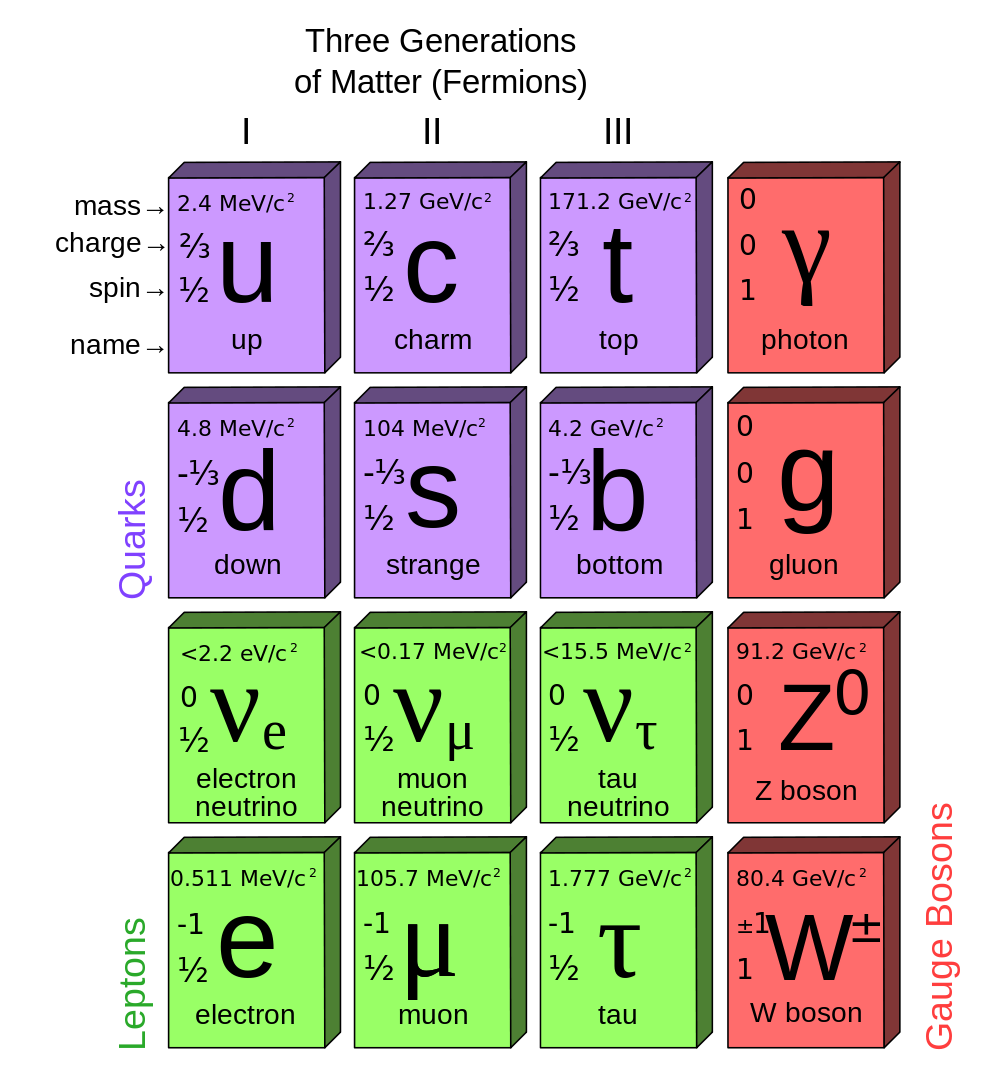
\includegraphics[width=.6\linewidth]{Introduction/figures/fundamentals.png}
\caption[Fundamental Particles of The Standard Model Before the LHC - FIND BETTER SOURCE]{The Fundamental Particles of the Standard Model and their Properties Before the LHC. Masses are listed in units of $eV/c^2$, a convenient unit for quantifying subatomic masses.}
\label{fig:fundamentals}
\end{center}
\end{figure}

Before the LHC was turned on, this (Fig~\ref{fig:fundamentals}) was the status of the observed particles and properties of the Standard Model. Absent from this picture is the Higgs boson. To understand the role of the Higgs boson and the importance of its discovery, we need to step back and motivate the Standard Model itself.

\subsection{The Story: The Status of the Standard Model Before the LHC}
\label{sec:SMpreLHC}

Trying to encapsulate the entire universe at once is undeniably intimidating. Fortunately, over centuries of development, physicists have established an arsenal of tools to make the task a bit more manageable. One of the most powerful techniques available is to locate and utilize a symmetry in the phenomenon to be considered; a planet should rotate around a star in the same fashion whether it's moving clockwise or counterclockwise. More than just identifying the symmetry to help simplify a problem, Noether's Theorem states if a system has a particular symmetry it inherently has an associated observed quantity. These examples are prolific, forming the basis of even introductory physics:

\begin{description}
\item[Conservation of Energy]
Time invariant Lagrangians\footnote{Lagrangians, referred to by $\Lagr$, are mathematical formulations which detail the dynamics of a given system.} conserve energy.
\item[Conservation of Momentum]
Translationally invariant Lagrangians conserve momentum.
\item[Conservation of Angular Momentum]
Rotationally invariant Lagrangians conserve angular momentum.
\end{description}

Symmetries themselves divide into two categories: global and local. Global symmetries apply to each point in the system equally, whereas local symmetries apply to individual points in the system. To picture the difference, imagine a grassy field where thousands of identical red balls have been placed in a grid. When you rotate all of the balls 10 degrees, this is a global transformation. If you rotate just one ball 10 degrees, this is a local transformation. In either case, the orientations of the balls will not appear to have changed, so the system has both a global and local symmetry.

The entire Standard Model can be described by only a few symmetries. Globally, the Standard Model obeys \textit{Poincar\'{e} symmetry}, which encapsulates all the symmetries we expect: translational (dynamics are invariant of location), rotational (dynamics unchanged by fixed rotation), time (dynamics will be identical regardless of when they start), and boosts (dynamics don't change if the whole system is moving at a uniform speed). Further, the Standard Model has three local symmetries which correspond to each of the three forces covered by the SM. Each of these local symmetries is called a {\it gauge symmetry} and has associated bosons called {\it gauge bosons} whose number is determined by the number of free parameters of the symmetry.

Electromagnetism, for example, has a gauge symmetry defined by U(1), the group associated with rotations about one axis. Since these rotations are only be defined by one angle, there should be just one gauge boson associated with electromagnetism. As explained in Sec.~\ref{sec:FundParticles}, the Standard Model has exactly that: the photon is this gauge boson. Indeed, gauge bosons are force carriers and vice versa. The weak force has a local symmetry of SU(2) and thus should have three gauge bosons\footnote{For brevity, the explanation for the number of bosons implied by SU(N) and the mathematics behind these groups are not provided, but detailed further in INSERT SU(N) REFERENCE}, which appear at first glance to match the $W^{\pm}$ and $Z$ bosons. The strong force has a local symmetry of SU(3) and has eight gauge bosons which match the eight gluons\footnote{Aside from a brief reprise dealing with hadronization in Sec.~\ref{sec:HadrCalo}, the strong force doesn't relate to the remainder of this thesis. Further information can be found at INSERT QCD REFERENCE}. Thus, we have our picture of fundamental fermions exchanging these gauge bosons to interact with one another.

However, mass has not yet been motivated. In fact, gauge bosons are mathematically required to be massless particles. Although the photon and the gluons are massless, why do the $W^{\pm}$ and $Z^{0}$ bosons have mass? The mass hierarchy of the fermions is also absent: if the top and up have otherwise identical properties, why is the top's mass over 75,000 times greater than the up? More problems arise: if matter and antimatter annihilate when they collide, why is there more matter than antimatter? And what about gravity? These are the deeper concerns of the Standard Model. Fortunately, there are answers that, if correct, could leave signatures we could find in particle accelerators.

\subsubsection{Searching for Professor Higgs' Boson}
\label{sec:findinghiggs}

Another common theme motivating the SM and physics beyond the SM is the idea of unification, all forces are simply different aspects of a single force. In 1961, Sheldon Glashow observed that electromagnetism and the weak force could be unified in the electroweak interaction~\cite{Glashow:1961}. In short, the unified U(1)$\times$SU(2) electroweak theory has one boson associated with U(1) ($B^{0}$) and three bosons associated with SU(2) (one neutrally charged $W^{0}$ and two charged bosons, $W^{+}$ and $W^{-}$). This symmetry is then broken such that the photon and $Z^{0}$ are mixtures of both the $B^{0}$ and $W^{0}$. Breaking a gauge invariance can introduce mass terms for the gauge bosons, so while the photon will be massless, the $W^{\pm}$ and $Z^{0}$ will be massive. This does provide the desired result, but it shifts the burden; there ought to be an explanation why this symmetry is broken. Shortly after this unification was proposed, a framework was proposed which explains how a gauge symmetry could be spontaneously broken instead of explicitly broken~\cite{Anderson:1963pc,Higgs:1964,Englert:1964,Higgs:1964-2,Guralnik:1964}: the \textit{Higgs Mechanism}. 

The Higgs mechanism details that there is a field that fills all of space and interacts with the particles of the Standard Model. How this gives a broken symmetry is best illustrated by looking at the associated potential. At high energies, we can picture the potential to be a symmetric valley centered around a point. In that case, the lowest energy state is stable and symmetric: if we imagine a ball rolling in such a structure, it would always come to the lowest point and the symmetry is preserved. But, as the universe cooled, the Higgs potential changed to what is seen in Fig.~\ref{fig:HiggsPotential}, commonly referred to as the ``Mexican-hat" or ``champagne bottle potential". As the ball started at the top of the bulge, it would fall to a lower energy state in the circular valley. Clearly, the symmetry that was preserved in the early universe would then be broken.

\begin{figure}[hbt]
\begin{center}
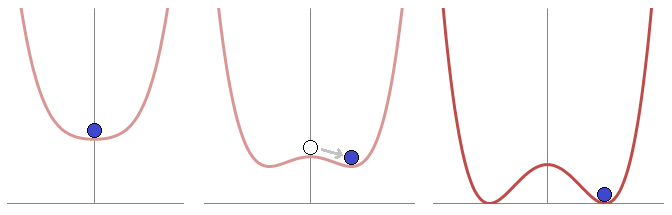
\includegraphics[width=.6\linewidth]{Introduction/figures/SpontaneousSymmetryBreaking.png}
\caption[The Higgs Mechanism - FROM WIKIPEDIA]{The Higgs Potential is a quartic potential with a negative quadratic term. This change in sign gives a ring of energetically favorable values, which provide the spontaneous symmetry breaking required by the Standard Model.}
\label{fig:HiggsPotential}
\end{center}
\end{figure}

This mechanism, along with the other fundamental forces and particles, was summarized into the Standard Model by Weinberg and Salam~\cite{Weinberg:1967,Salam:1968}. In doing so, we have a natural explanation for the massless photon and massive $W^{\pm}$ and $Z^{0}$ that we require. The massive $Z^{0}$ in particular had only been predicted when the Standard Model was finalized in the late 1960s, but in the coming decades it was observed indirectly in the 1970s~\cite{} and then directly in the 1980s~\cite{}. On top of making the $W^{\pm}$ and $Z^{0}$ massive, by breaking the Electroweak symmetry fermions acquire a mass proportional to how strongly they couple to the Higgs field. This explains why the top and the up have such greatly differing masses.

Crucially, the completion of the Standard Model with the Higgs mechanism from an experimental perspective is to confirm that the Higgs field exists and does generate the masses as described. The final prediction of the Standard Model is that there should be excitations of the Higgs field which manifest as the \textit{Higgs boson}, commonly shortened to just ``the Higgs", which is an uncharged zero-spin particle. The strength that bosons and fermions couple to the Higgs field is only determined by the mass of the Higgs boson, so the only unknown in the SM before the LHC was what this mass is.

Before the LHC, all attempts to find the Higgs boson had been elusive. Theoretically, $m_{H}\lesssim1$~TeV otherwise there would be large instabilities in the universe that would have already been observed~\cite{}. A lower bound on the Higgs mass was set at LEP, an electron-positron collider, where $m_{H}>114.4$~GeV~\cite{Barate:2003sz} at the 95\% confidence level. From measuring properties of the SM to higher and higher precision, the Higgs mass was expected to be found in the mass range $m_{H}\lesssim185GeV$. Since the exact Higgs mass was not known and these excitations should be extraordinarily rare, the best chance to find the predicted Higgs would be a general purpose detector at a particle accelerator that scans a wide range of energies with a very high throughput. The Tevatron is such a collider and its general detectors, D0 and CDF, further excluded the Higgs from having a mass between $160<m_{H}<170$~GeV~\cite{Aaltonen:2010yv}, leading to the status showing in Fig.~\ref{fig:HiggsExclusionPreLHC} In Sec.~\ref{sec:expt}, we argue that the CMS detector at the LHC is ideal for extending this search.

\begin{figure}[hbt]
\begin{center}
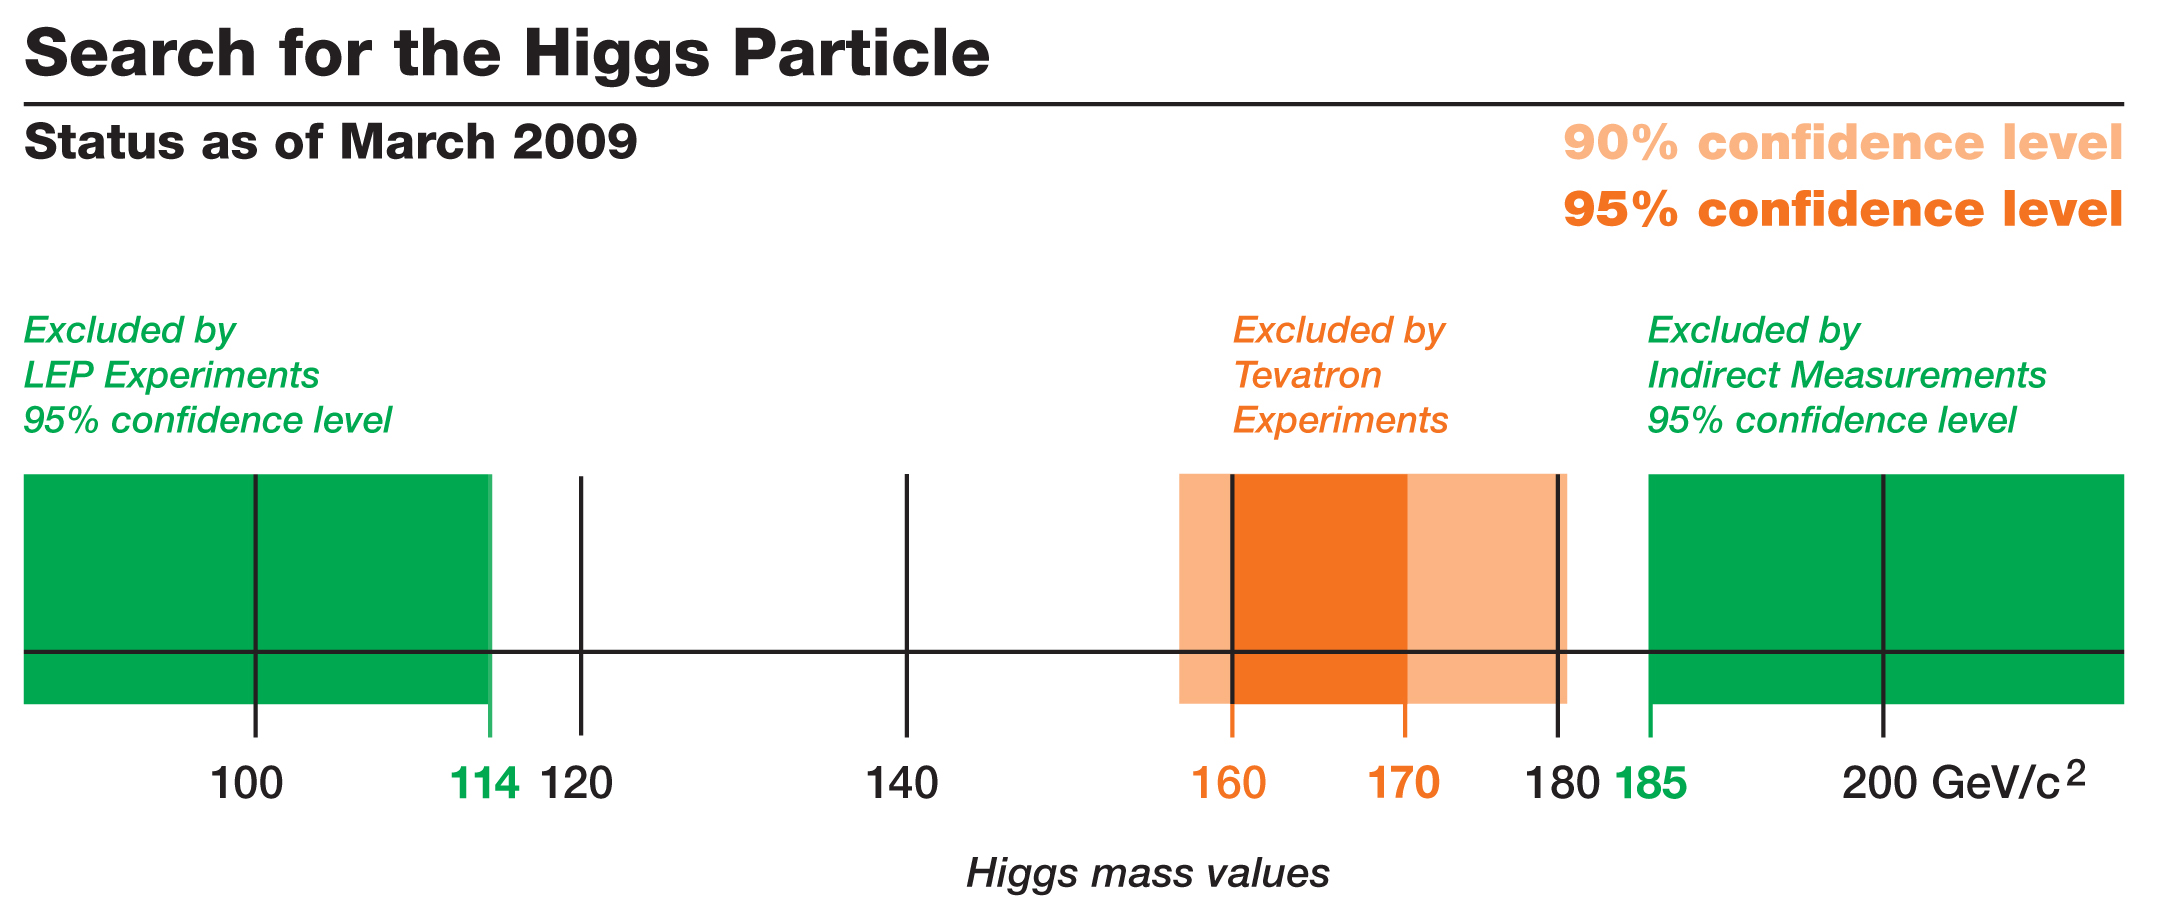
\includegraphics[width=.6\linewidth]{Introduction/figures/HiggsExclusions_09.jpg}
\caption[Higgs Mass Limits Before the LHC]{Before the LHC, the Higgs Boson's mass was excluded to 95\% confidence in the ranges $m_{H}<114.4$~GeV, $160<m_{H}<170$~GeV, and $m_{H}>185$~GeV.}
\label{fig:HiggsExclusionPreLHC}
\end{center}
\end{figure}

\subsubsection{Expecting the Unexpected}
\label{sec:findingBSM}

Adding the Higgs Boson to our cast of fundamental particles completes the Standard Model, but there are still remaining difficulties:

\begin{description}
\item[Matter v Antimatter] \hfill \\
Matter and antimatter annihilate when they interact, yet the visible universe is largely made of matter. The current theoretical explanation for this asymmetry is that there are particles and decays that would have a preference for matter over antimatter~\cite{}. Although some of this asymmetry has been predicted and observed, neither are sufficient to account for the relative lack of antimatter.
\item[Gravity] \hfill \\
Gravity is notoriously absent from the SM. Its inclusion is extraordinarily difficult. Gravity is many orders of magnitude weaker than any of the other three forces and must appear like General Relativity at large distances, but currently quantum models of gravity break down at very small distances.
\item[Neutrino Masses] \hfill \\
In the SM, neutrinos are not predicted to have mass, yet they have been observed to oscillate between different generations~\cite{}. In order to account for these oscillations, the neutrinos are required to have different masses and thus must be massive.
\item[Dark Matter and Dark Energy] \hfill \\
Current estimates of the universe say that only 4\% of all mass-energy is made of the particles in the Standard Model. The remaining 96\% is made up of Dark Matter (23\%) which seems to only interact gravitationally and Dark Energy (73\%) which is responsible for the acceleration of the expansion of the universe.
\end{description}

These questions lead to models that are considered Beyond the Standard Model (BSM) physics. There are two main veins of BSM physics, Supersymmetry (SUSY) and Extra Dimensions. As discussed already, symmetry is a very powerful tool in theoretical physics. SUSY takes the symmetries available under the SM and adds one additional symmetry which predicts new supersymmetric partners for every particle in the SM. For example, every fermion will have a supersymmetric bosonic partner, e.g. the selectron to the electron or the sbottom to the bottom. These partners could provide answers for some or all of the unresolved questions in the SM. Extra dimensions posits that beyond the four traditional dimensions, three spatial and one time, there are additional dimensions which are not readily observed. Additional particles and properties can be hidden in excitations of these extra dimensions which could also explain these unresolved questions.

These additional particles and properties influence searches at the LHC aside from direct observation. First and foremost, nearly all BSM models would require not just one but multiple Higgs bosons, any or all of which could be probed at the LHC. Thus, even though the Higgs of the SM is most likely to be found in the mass range $<m_{H}<$, the search should be extended to look for other resonances which may be Higgs-like that would give credence to BSM physics. Furthermore, each of these particles could have different properties than what we expect in the SM Higgs mechanism. Many theorized explanations of gravity imply the existence of another boson called the graviton. Such a particle would have spin-2 instead of the spin-0 presumed in the SM Higgs, so it is also important to probe the spin of any new particle.

Some new physics comes from looking at high precision measurements which predicate the discovery of undiscovered fundamental particles, as was predicted with the $Z^{0}$. For example to achieve the matter/antimatter asymmetry, there need to be particles that violate CP-symmetry, where a system's dynamics are identical if all matter is replaced with antimatter (and vice versa) and the spatial coordinates are inverted. Given that the CP-symmetry needed to explain the matter/antimatter asymmetry has not yet been observed, the hope is that new particles would break this symmetry. Even if no other particles aside from a Higgs candidate are found, the SM Higgs is predicted to preserve this symmetry (\textit{CP-even}) and any deviation in the properties from the expected could prove invaluable towards future research into the field of particle physics.

\section{Summary}
\label{sec:intro_summary}

As previously mentioned, we now know that there is a Higgs boson, but it is insightful in retrospect to walk through the discovery chronologically to understand the process and appreciate its significance. In Sec.~\ref{sec:expt}, the LHC will be expounded, particularly the CMS experiment and how it was designed to look for a Higgs boson or other new physics. In Sec.~\ref{sec:pheno}, one possible signature of the Higgs will be investigated, including why it is considered the ``golden" channel and how it has been crucial to the discovery of the boson and its properties. In Sec.~\ref{sec:results}, the observed properties will be detailed and how well they match up with what we expect in the Standard Model. Lastly, in Sec.~\ref{sec:conclusions}, the effects of these results will be summarized and what they mean for future measurements.
\chapter{Experimental Setup}
\label{sec:expt}
\chaptermark{Experimental Setup}

\begin{center}
\begin{footnotesize}
{\it{``I'm going to find it and I'm going to destroy it. I don't know how yet. Maybe dynamite."}}\\
Steve Zissou, ``The Life Aquatic with Steve Zissou"
\end{footnotesize}
\end{center}

\section{The Large Hadron Collider}
\label{sec:LHC}

In Sec.~\ref{sec:introduction}, we saw that although the Standard Model was tested robustly before the LHC turned on, the Higgs boson had not yet been discovered and there are still unanswered questions not covered under the Standard Model that should lead to new physics. For many decades, the primary tool of discovery in experimental particle physics has been the particle accelerator. In rudimentary terms, two particles are accelerated towards each other and the byproducts of their collisions are studied to look for new particles.

There are two categories of particle accelerators, leptonic and hadronic: leptonic colliders have electron-positron collisions while hadronic colliders use proton-proton or proton-antiproton collisions. As discussed in Sec.~\ref{sec:FundParticles}, protons are made up of a sea of different particles with varying energies, making it difficult to know the exact initial conditions of a collision. A leptonic collider, on the other hand, can tune the initial energy of the collisions to a precise value with strictly designed initial conditions. However, as argued in Sec.~\ref{sec:findinghiggs} and \ref{sec:findingBSM}, the proposed particles could take many energy values, so any search must be done over a wide range, which encourages the use of hadronic collisions. Furthermore, this energy range should explore unprobed regions out of reach of previous detectors. The highest energy collision before the LHC were at the Tevatron at Fermilab which had a maximum center-of-mass energy up to about 2 TeV (2000 GeV).

The Large Hadron Collider was designed with these characteristics in mind: a 27-kilometer circular accelerator for proton-proton\footnote{Heavy ions can also be accelerated in the LHC, leading to interesting research for the strong force, but this is outside the scope of this thesis.} collisions that can reach up to energies of 14 $\rm{TeV}$. An earlier proton-proton accelerator, the Super Proton Synchrotron which found direct evidence for the $Z$ boson~\cite{Arnison:1983rp,Arnison:1983mk,Bagnaia:1983zx}, initializes the proton bunches at 450 $\rm{GeV}$ for injection into the larger ring. Once reaching the LHC, a series of 1232 superconducting dipole magnets with radio frequency cavities increase the energy of the protons as they move around the ring. As these bunches accelerate, the protons will tend to diffuse, so thousands of additional magnets (quadrupole, octopole, etc) are installed to focus the beam. Each bunch in the LHC contains $1.15\times10^{11}$ protons and every run contains 2808 bunches. These high populations are required to probe the highest energies and rarest interactions expected at the LHC.

To quantify how rare an event is, physics utilizes the concept of \textit{cross section} ($\sigma$). This is best illustrated by comparing protons in a bunch to a flow of ballbearings: as two bunches pass through one another, the likelihood that any ballbearing strikes another is proportional to their size, literally their cross-sectional area. Similarly, in quantum physics, the likelihood of an event is determined by its cross section, typically written in units of \textit{barns} (b) where $1$ $\mathrm{b}$ $=$ $10^{-28}$ $\mathrm{m}^2$. The processes intended to be probed at the LHC have cross sections ranging from the order of picobarns ($1$ $\mathrm{pb}$ $=$ $10^{-12}$ $\mathrm{b}$) to fractions of femtobarns ($1$ $\mathrm{fb}$ $=$ $10^{-15}$ $\mathrm{b}$).

Particle accelerators use \textit{luminosity} ($\mathcal{L}$) to indicate how many events of a given cross-section should be expected per second, i.e. $\frac{dN}{dt}=\mathcal{L}\times\sigma$. The luminosity can be defined in terms of the accelerator's parameters:
\begin{equation*}
\mathcal{L} = \frac{\gamma f k_{B}N_p^2}{4\pi \epsilon_{n} \beta^{*}}F
\end{equation*}
where $\gamma$ is the Lorentz factor corresponding to how fast the particles are moving, $f$ is the frequency that bunches revolve through the LHC, $k_{B}$ is the number of bunches, $N_p$ is the number of protons in a bunch, $\epsilon_n$ (normalized transverse emittance) and $\beta^{*}$ (betatron function at the point of interaction) both relate to the physical size of the beam, and $F$ is a reduction factor caused by the crossing angle of the beams. Relevant design parameters are also found in Table~\ref{tbl:LHCLumi}. Ultimately, the design luminosity of the LHC is $\mathcal{L} = 10^{34}$ $\mathrm{cm}^{-2}\mathrm{s}^{-1}$ which corresponds to about 1 billion proton-proton interactions per second. To quantify the total amount of data collected by a particle detector, time-integrated luminosity, in units of $fb^{-1}$, is used to gauge how many events of a given cross-section should be expected. For example, with 10 $\mathrm{fb}^{-1}$ of data, one would expect 10 events for a cross-section of 1 $\mathrm{fb}$.

\begin{table}[htp]
\begin{center}
\begin{tabular}{|c|c|c|}
\hline
Number of bunches & $k_B$ & 2808 \\
\hline
Number of protons/bunch & $N_p$ & $1.15\times10^{11}$ \\
\hline
Bunch separation & & 25 ns \\
\hline
%Betatron Function at IP & $\beta^{*}$ & 0.55 m \\
%\hline
%Normalized Transverse Emittance & $\epsilon_n$ & 3.75 $\mu\mathrm{m}$ \\
%\hline 
Design Luminosity & $\mathcal{L}$ & $10^{34}$ $\mathrm{cm}^{-2}\mathrm{s}^{-1}$ \\
\hline
\end{tabular}
\caption{Design Parameters of the LHC}
\end{center}
\label{tbl:LHCLumi}
\end{table}%

After reaching the desired energy, the proton bunches can interact at four crossing points. Each of these points is the site of a detector on the LHC: CMS (The \textbf{C}ompact \textbf{M}uon \textbf{S}olenoid), ATLAS (\textbf{A} \textbf{T}oroidal \textbf{L}HC \textbf{A}pparatu\textbf{s}), ALICE (\textbf{A} \textbf{L}arge \textbf{I}on \textbf{C}ollider \textbf{E}xperiment), and LHCb (\textbf{LHC} \textbf{b}eauty Experiment). CMS and ATLAS are general detectors for proton-proton interactions, while ALICE and LHCb use the protons to collide with heavy-ion targets to look deeper into the intricacies of the strong force. The remainder of this chapter will detail CMS and how it is used to search for particles like the Higgs.

\section{Our Setting: The Compact Muon Solenoid}
\label{sec:CMS}

The Higgs Boson and theorized particles in BSM physics are expected to be unstable and rapidly decay to particles of the Standard Model, so it's unsurprising that the design requirements of the CMS are built around accurately detecting these particles and characterizing their energies and momenta. To collect the most information about these events, a detector should be designed to record all decay chains so that the full kinematics could be reconstructed. This is the idea behind a \textit{hermetic} detector: different subsystems are nested to capture information about any particle observed and characterized by what sub-detectors they interact with. A detailed view of the CMS detector is seen in Figure~\ref{fig:ExplodedCMS}. This section will overview the subsystems, where further details are found in the CMS Technical Design Reports~\cite{CMSTDR:Vol1,CMSTDR:Vol2}.

\begin{figure}[htbp]
\begin{center}
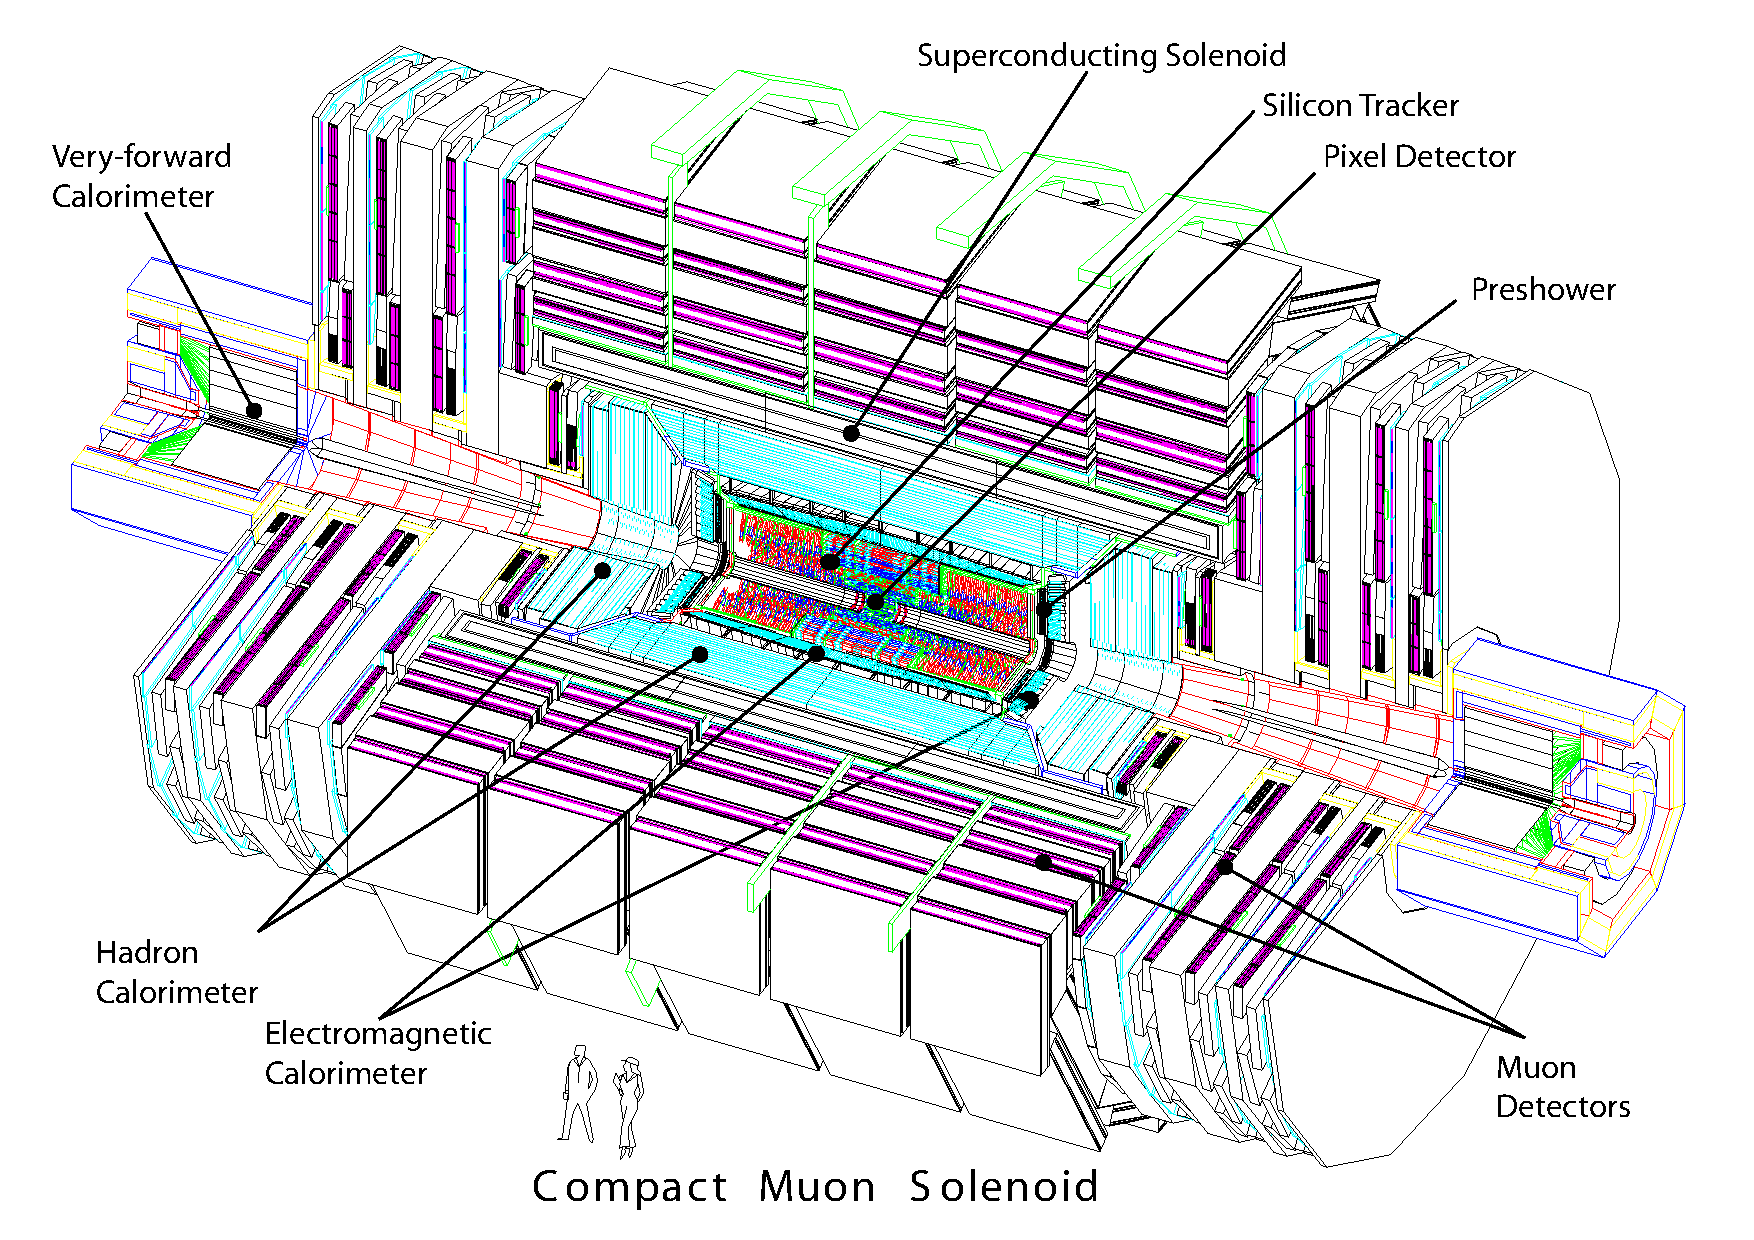
\includegraphics[width=.9\linewidth]{Experiment/figures/ExplodedCMS.pdf}
\caption[The CMS Detector with Sub-Detector Systems]{The CMS detector is built around a superconducting solenoid, with the muon system (Sec.~\ref{sec:MuonSystem}) on the outer shell. Inside the solenoid, the silicon tracker and pixel detector (Sec.~\ref{sec:Tracker}) are at the innermost radii, with the calorimeter systems (Sec.~\ref{sec:ElecCalo} and \ref{HadrCalo}) are close to the solenoid. Two human figures are used for scale.}
\label{fig:ExplodedCMS}
\end{center}
\end{figure}

\subsection{Coordinates and Conventions for the CMS}
\label{sec:CoordinateConventions}

To unambiguously define locations for components or events found in the detector, a standard coordinate system is used such that the origin is centered at the nominal collision point. In cartesian coordinates, the $y$-axis is defined to be vertically upward while the $x$-axis is points toward the center of the LHC accelerator ring. However, given that the detector is cylindrically symmetric, directions are commonly defined using $\phi$ and $\eta$. $\phi$ is the azimuthal angle starting from the $x$-axis in the $x-y$ plane. $\eta$ is the \textit{pseudorapidity} where $\eta=-\ln[\tan(\theta/2)]$, $\theta$ being the polar angle measured from the $z$-axis. Momentum and energy are then broken into their transverse (away from the axis, e.g. $p_T,E_T$) and longitudinal (along the axis, e.g. $p_z,E_z$) components. Given that the beam is very near the axis and would cause a sizable background, particles that have large $p_T$ or $E_T$ (or in the case of searching for energy imbalance, $E_T^{miss}$) should be the easiest to identify unambiguously.

\subsection{Subsystems in CMS}
\label{sec:CMSSubsystem}

\subsubsection{The Magnet}
\label{sec:Magnet}

One way to categorize the decay products of a particle is to look at their charges. Any charged particle will have a curved trajectory in a magnetic field, where the direction of curvature is determined by the sign of the charge and its scale is proportional to the momentum. Given the large energies and desired precision of the momenta, the magnetic field must be very strong and consistent. CMS uses a 12.9m long, 5.9m in diameter superconducting solenoid with a designed field strength of 4T, about 100,000 times that of the Earth's magnetic field. An iron return yoke, running through the muon system, is used to guide and return the field. In doing so, the magnetic field in the muon system will be antiparallel and of lower magnitude than the field in the calorimeters and tracking systems.

\subsubsection{Muon System}
\label{sec:MuonSystem}

Muons are one of the cleanest signatures to identify and thus crucial for finding new physics. For charged particles, electrons are common byproducts of many low energy decays and can be stopped in dense material. Tau leptons are much rarer, but have a very short lifetime and thus decay in the inner detector. Quarks cannot be observed individually. Neutrinos aren't charged and very difficult to detect as they only interact via the weak force. Muons, on the other hand, are charged, heavy leptons that have long enough lifetimes to pass through the outer reaches of the detector. Because of these properties\footnote{For exactly the same reason, this is why the LHC is deep underground. Cosmic rays commonly hit the Earth's atmosphere and shower particles to the surface. Although nearly all particles can be shielded without much material, decay in the upper atmosphere, or very rarely interact with matter, muons will commonly penetrate the surface and need hundreds of meters of depth to suitably reduce this background.}, muons that come from collisions are measured from three different sub-systems to accurately measure their kinematics. 

\begin{figure}[htbp]
\begin{center}
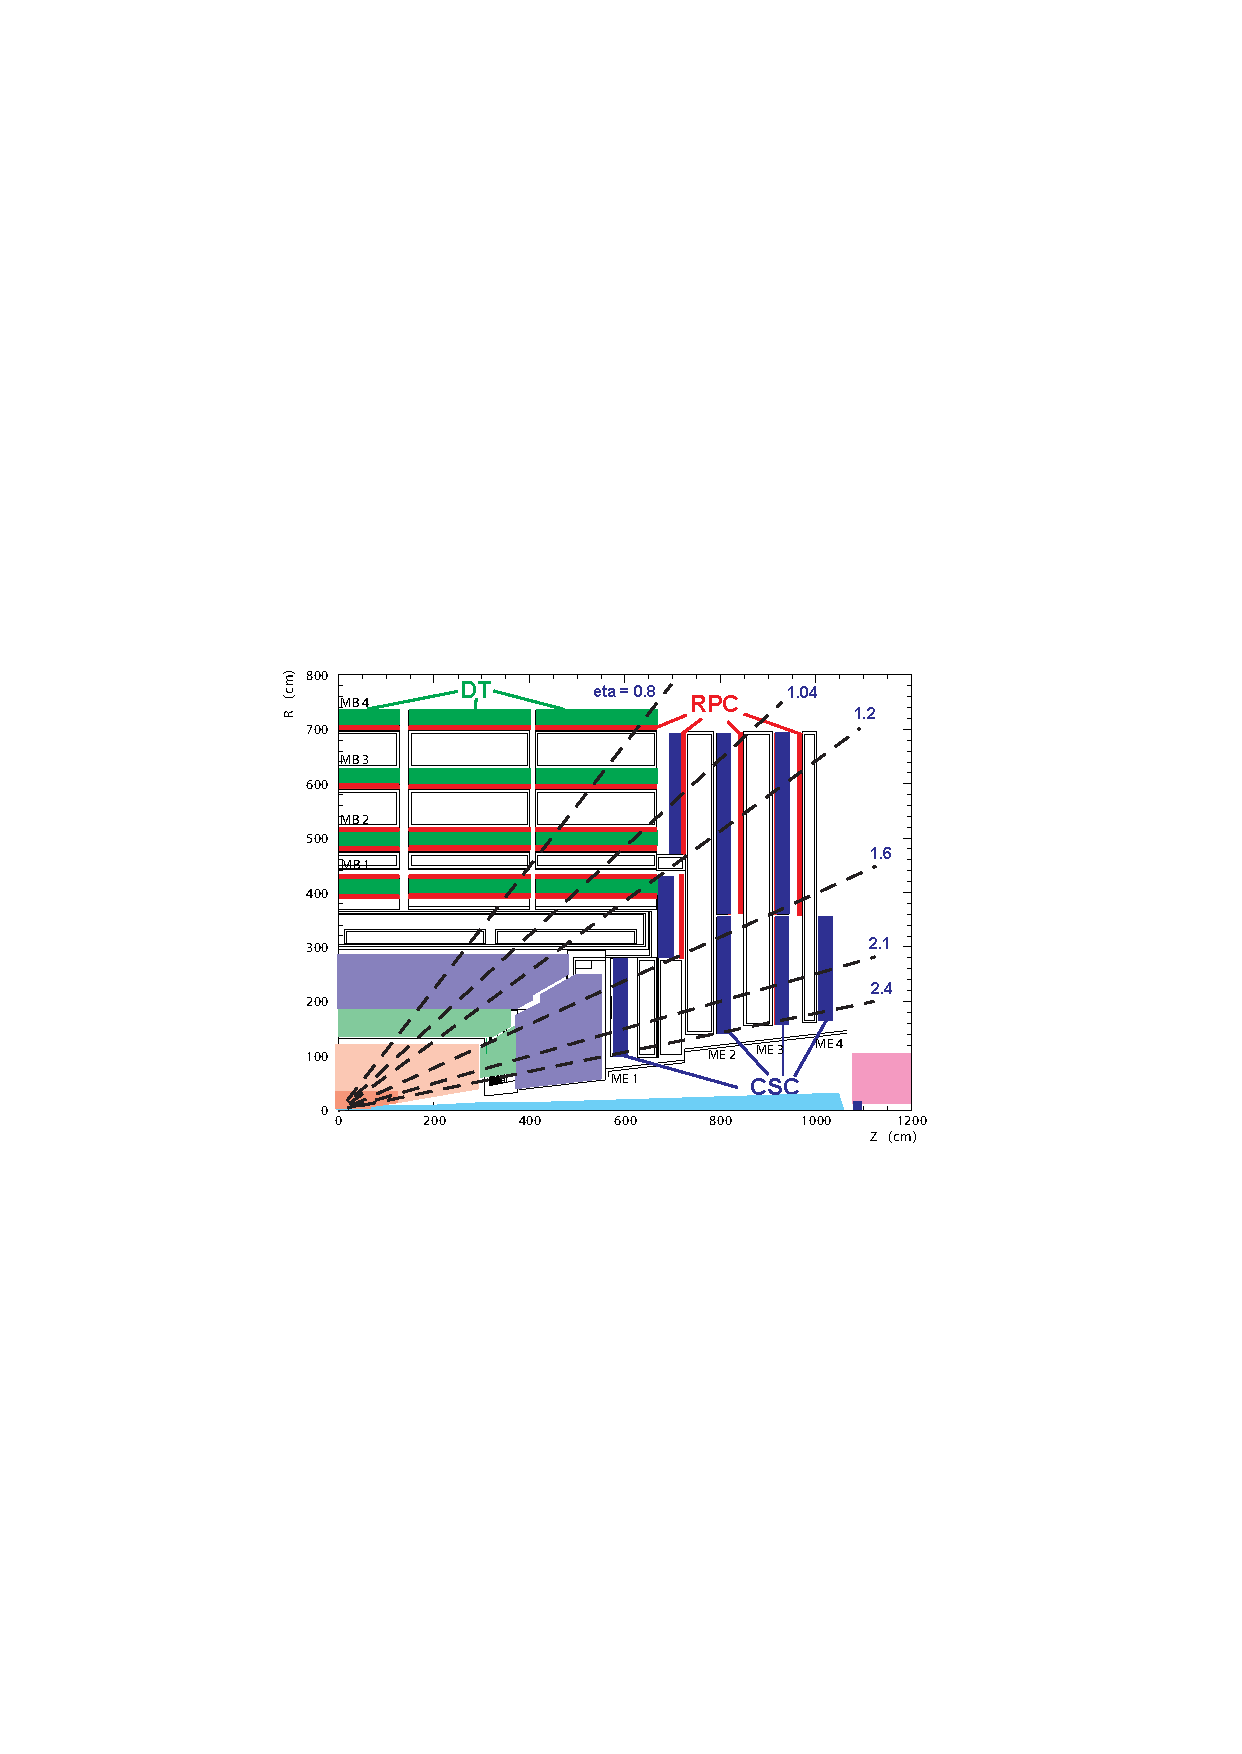
\includegraphics[width=.7\linewidth]{Experiment/figures/MuonSystem.pdf}
\caption[Arrangement of Detectors in CMS Muon System]{Vertical slice of CMS showing one quarter of the muon system. The three different devices used are labeled: Drift Tube (DT) chambers, Cathode Strip Chambers (CSC), and Resistive Plate Chambers (RPC).}
\label{fig:MuonSystem}
\end{center}
\end{figure}

On the outer edge of the detector, three types of detectors are used to measure muons. The layout of the different types of detectors can be seen in Fig.~\ref{fig:MuonSystem}. Away from the beam line ($|\eta|<1.2$), along the barrel, four layers of 250 drift tube (DT) chambers are used. Each chamber is composed of a positively charged wire in a volume filled with gas. As a muon moves through the chamber, the gas becomes ionized and the freed electrons will drift toward the wire. The position of the muon can then be tracked by where electrons were observed to drift. Closer to the beam line (up to $|\eta|<2.4$), in the endcaps, there are four layers of 468 trapezoidal shaped cathode strip chambers (CSC). Each CSC is made of seven layers of metal, inlaid with a plane of cathode strips plus anode wires nearly perpendicular to the strips. The gaps between metal layers are filled with a gas that will ionize when any charged particle passes through, causing an electron avalanche. Similar to the DTs, these electrons will charge anode wires and cathode strips near the trajectory, allowing spatial reconstruction at each layer.

Finally, in both the barrel and endcap regions ($|\eta|<1.6$), 1080 resistive plate chambers (RPC) are added in conjunction with the DTs or CSCs. Each RPC consists of two very narrow chambers (2mm thick x 130cm long) filled with gas plus anode and cathode plates made of bakelite, which has a very high resistivity. As with DTs or CSCs, when charged particles pass through the gas, it ionizes and is quickly detected with the bakelite layers. By design, RPCs have worse spatial resolution than either the DTs or CSCs, but their response is much faster with high time resolution, allowing for very rapid identification of muons. This will prove particularly relevant to triggering at CMS in Sec.~\ref{sec:Triggers}.

By tracking the muons through these different detectors, their trajectories, and thus their momentum, can be reconstructed. When combined with the inner tracker (see Sec.~\ref{sec:Tracker}), the overall resolution is well below 10\% across all expected momenta near the barrel and most momenta ($p \lesssim 2 \rm{TeV}/c$) in the endcaps, as seen in Fig.~\ref{fig:MuonMomentumResolution}.

\begin{figure}[htbp]
\begin{center}
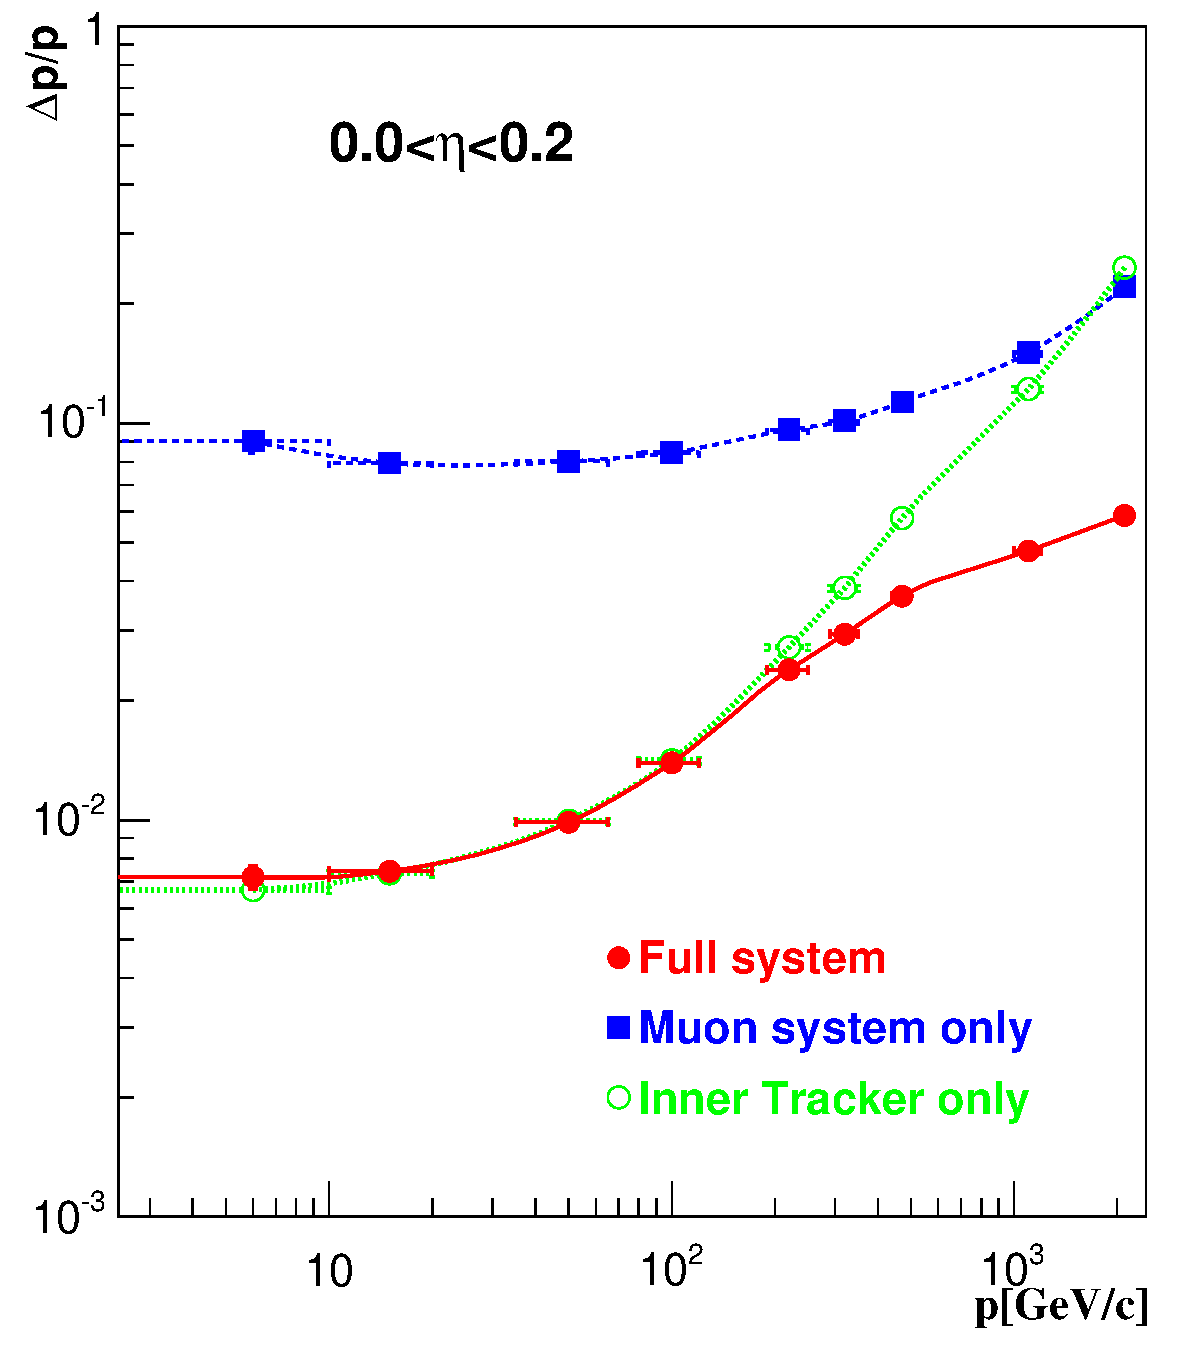
\includegraphics[width=.45\linewidth]{Experiment/figures/MuonMomentumResolution_smalleta.pdf}
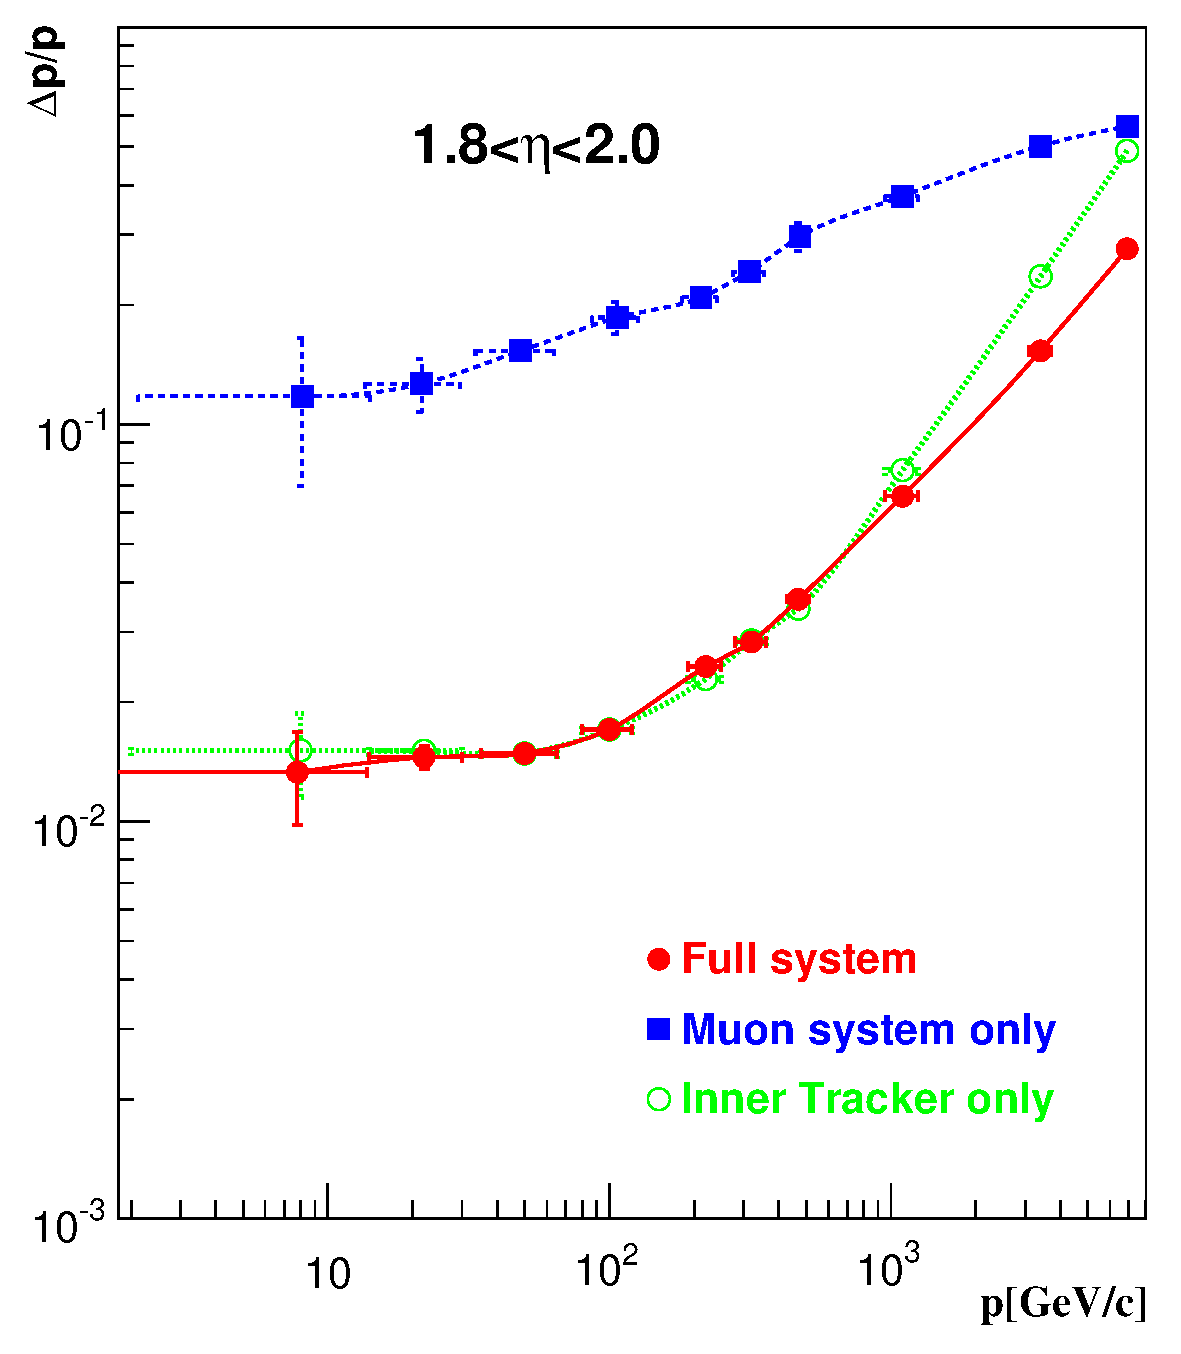
\includegraphics[width=.45\linewidth]{Experiment/figures/MuonMomentumResolution_higheta.pdf}
\caption[Muon Momentum Resolution at CMS]{Momentum resolution of muons for the muon system only, inner tracker only, or both in the barrel (left) and endcap (right) regions.}
\label{fig:MuonMomentumResolution}
\end{center}
\end{figure}


\subsubsection{Electromagnetic Calorimeter}
\label{sec:ElecCalo}

In order to detect particle energies at CMS, an electromagnetic calorimeter (ECAL) made of lead tungstate ($\rm{PbWO}_4$) barrel crystals (61200 such crystals in the barrel [$0<|\eta|<1.479$], 7324 in the endcaps [$1.479<|\eta|<3.0$]) is built just outside of the inner tracking system. As the name implies, this sub-detector is designed to detect particles that predominantly interact electromagnetically, namely photons and electrons. As photons and electrons pass through a dense transparent material, they will interact with the heavy nuclei therein. Electrons have their paths diverted by the strongly positively charged nuclei in a process called \textit{bremsstrahlung}, where the diversion will emit a photon. Meanwhile, photons of a sufficient energy can \textit{pair produce} in the presence of a heavy nucleus, decaying into an electron and positron pair. Muons, taus, and most particles coming from strong processes are typically too heavy or interact too weakly to initiate these decays, so they will pass through the ECAL.

The combination of these processes produce showers of electrons and photons of lower energy. This showering has two characteristic length scales. The radiation length, $X_0$, determines the depth of a shower in the calorimeter while the Moliere radius determines a shower's width. Lead tungstate was chosen explicitly because it has short radiation and Moliere lengths (0.89 cm and 2.2 cm, respectively) while maintaining a fast response time roughly equal to the bunch crossing time. Each of the crystals in the ECAL have a square front facing cross-section (about $22\times22$ $\rm{mm}^2$ and $28.6\times28.6$ $\rm{mm}^2$ for the barrel and endcaps, respectively) with a length equal to a large number of radiation lengths (25.8$X_0$ for the barrel, 24.7$X_0$ for the endcap) so these electromagnetic showers are fully contained in the ECAL. 

Particles that deposit their energy in the ECAL can then be measured by adding the energies of the resultant shower products. However, electromagnetic showers in lead tungstate will yield a small number of total photons, only about 4.5 photoelectrons per MeV reach the end of the crystal, so additional electronics are placed to act as photodetectors and amplify the signals. In the barrel, two silicon avalanche photodiodes (APDs) are attached to the far end of each crystal, while vacuum phototriodes (VPTs) are at the end of each endcap crystal. Both the crystals and the APDs are highly sensitive to temperature changes, so the ECAL requires a cooling system to maintain temperature stability. 

To test the performance of the crystals, the performance of a supermodule of crystals was measured with a test electron beam before installation. The energy resolution was then parameterized as a function of energy:
\begin{equation}
\left(\frac{\sigma}{E}\right)^2 = \left(\frac{S}{\sqrt{E}}\right)^2 + \left(\frac{N}{E}\right)^2 + C^2
\end{equation}
where $S$ is the stochastic term coming from random statistical fluctuations, $N$ is the noise from the detector, and $C$ is a constant term. The values of the parameters and this parameterization as a function of energy are found in Fig.~\ref{fig:ECALResolution}.

\begin{figure}[htbp]
\begin{center}
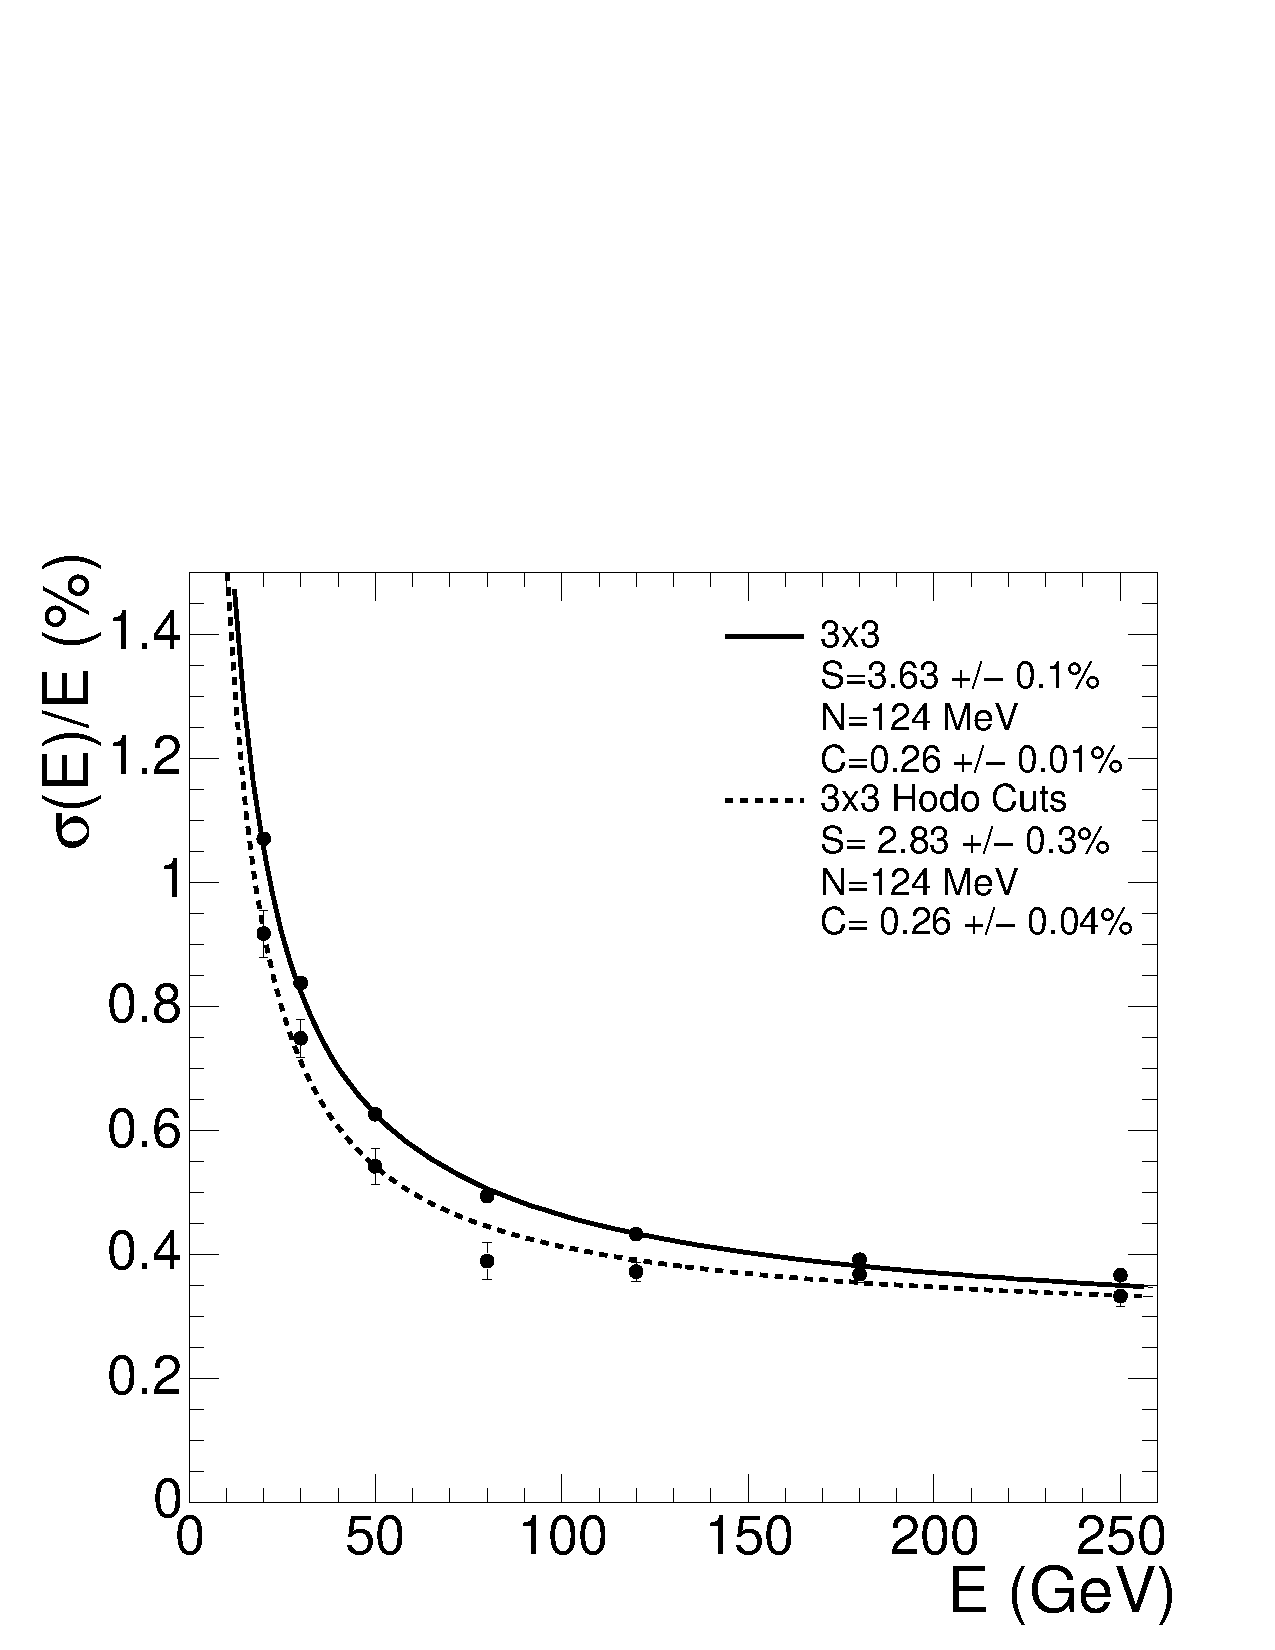
\includegraphics[width=.7\linewidth]{Experiment/figures/ECALResolution.pdf}
\caption[Resolution of the Electromagnetic Calorimeter as a Function of Energy]{ECAL Supermodule Energy Resolution, $\sigma(E)/E$ as a function of the electron energy from the test beam. The solid and dashed lines vary by the area used to reconstruct the energy.}
\label{fig:ECALResolution}
\end{center}
\end{figure}

\subsubsection{Hadronic Calorimeter}
\label{sec:HadrCalo}

For non-muonic particles that pass through the ECAL, another calorimeter is needed to measure the energy of the hadronic products of CMS, called the hadronic calorimeter (HCAL). As mentioned in Sec.~\ref{sec:FundParticles}, quarks and gluons cannot be observed in an isolated state, instead being found grouped into hadrons. At particle accelerators, these hadrons will have a sufficiently high momentum that the constituents will pull apart from one another. However, a property of the strong force is that as two colored particles move apart, the energy of the bond between the particles will increase. This means that at some distance, it becomes energetically favorable for the hadron to split into a pair of hadrons. Simultaneously, the quark or gluon constituents may radiate lower energy gluons, which will similarly tend to split into quarks or gluons. These processes are termed \textit{hadronization} and \textit{fragmentation}, where the end result is analogous to the electromagnetic case: bare quarks and gluons will appear as showers of hadrons and their decays products. These showers are called \textit{jets}.

While the ECAL was made of continuous crystals that could generate and direct the resultant particles to detecting elements, the HCAL uses sampling. When jets strike a dense material with a suitably short interaction length, there will be some decay in this absorber layer. Then, these particles pass through a plastic scintillator where the decay products will radiate high frequency photons according to their energy. By alternating these layers, the energy of a jet can be found through multiple samples, effectively making energy snapshots of the decay.

In the barrel region ($|\eta|<1.4$)\footnote{There is also a hadron outer detector in the barrel $|\eta|<1.26$ in the muon system that sample the energy penetrating from hadronic showers to reduce contamination.}, there are 32 such layers\footnote{Their thicknesses are identical except the first layer which is thicker to account for particles that leave the ECAL.}, segmented into towers of $\Delta\eta\times\Delta\phi = 0.087\times0.087$. The absorber layer is made of brass due to its non-magnetic properties and short interaction length. Each scintillating element is embedded with wavelength-shifting fibres which carry the light to multi-channel hybrid photodiodes (HPDs) which apply a gain to the photoelectrons to find the corresponding energy. In the endcap ($1.3<|\eta|<3.0$), there are 14 layers identical to the barrel region but with slightly different segmentation ($\Delta\eta\times\Delta\phi = 0.087\times5^{\circ}$ for small $|\eta|$ to $\Delta\phi=10^{\circ}$ with $0.09<\Delta\eta<0.35$ for larger $|\eta|$). Finally, there is also a hadron forward (HF) calorimeter ($3.0<|\eta|<5.0$) built of absorbing layers of steel and quartz fibres, which scintillates and directs light to photomultipliers, segmented into elements of $\Delta\eta\times\Delta\phi \approx 0.175\times10^{\circ}$. A sample output of the HCAL can be seen in Fig.~\ref{fig:HCALOutput} while jet energy resolution can be found in Fig.~\ref{fig:HCALResolution}.

\begin{figure}[htbp]
\begin{center}
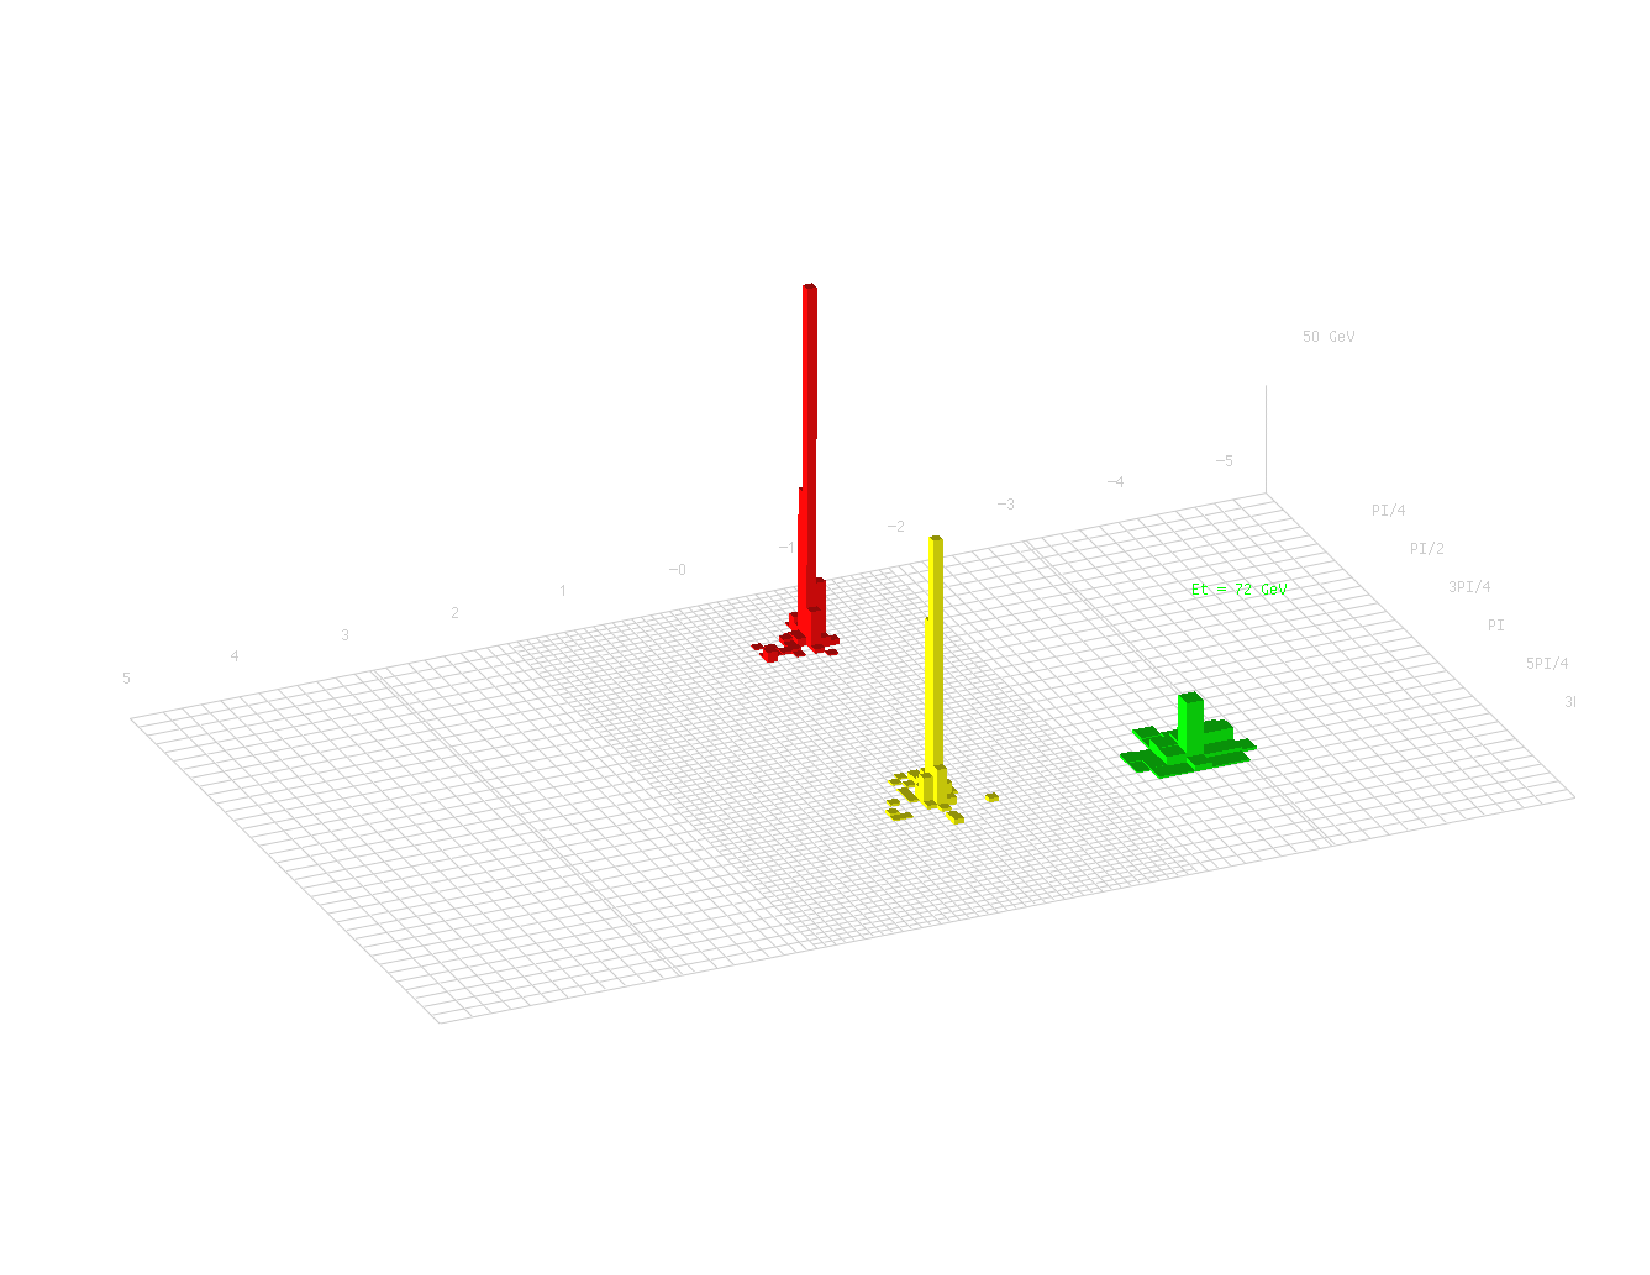
\includegraphics[width=.7\linewidth]{Experiment/figures/HCALOutput.pdf}
\caption[Sample Output of the Hadronic Calorimeter]{Multi-jet event in the HCAL, showing the $\eta,\phi$ segmentation over the full range ($0\leq\phi<2\pi$, $-5.0<\eta<5.0$). Heights correspond to the energy recorded in a particular tower of segments.}
\label{fig:HCALOutput}
\end{center}
\end{figure}

\begin{figure}[htbp]
\begin{center}
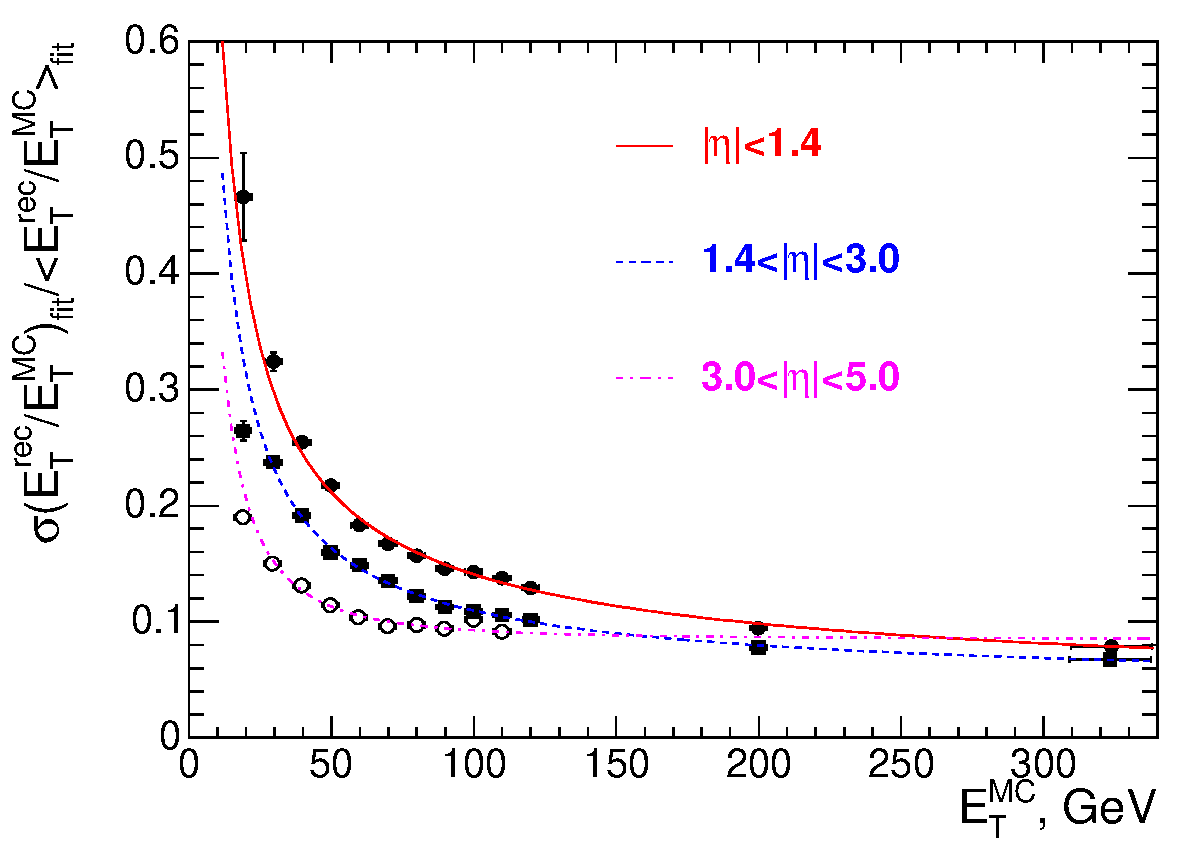
\includegraphics[width=.7\linewidth]{Experiment/figures/HCALResolution.pdf}
\caption[Resolution of the Hadronic Calorimeter as a Function of Simulated Transverse Energy]{Resolution of the transverse energy of jets as a function of the simulated jet energy, discriminated by barrel ($|\eta|<1.4$), endcap ($1.4<|\eta|<3.0$), and forward ($3.0<|\eta|<5.0$) regions of the hadronic calorimeter (HCAL).}
\label{fig:HCALResolution}
\end{center}
\end{figure}

By unifying the information from the ECAL, HCAL, and Muon systems, CMS can fully detail the energies of all decay products. The only particles of the Standard Model not detected by these systems are neutrinos, which will pass through the detector. However, by the hermetic design of CMS, neutrinos can be accounted for in a given interaction by looking at the missing energy in a given event\footnote{Searches are also done looking for anomalously large amounts of missing energy which could account for any number of BSM physics, including microscopic black holes, extra dimensions, weakly interacting massive particles, etc. However, as of writing, no new physics has been observed in these searches.}. 

\subsubsection{Inner Tracking System}
\label{sec:Tracker}

While other subsystems are built primarily to measure the energies of the particles in a given event, the momentum of the particles must also be measured to very high precision so that the full kinematics can be determined. To do this, CMS uses a tracker system, which uses combinations of silicon pixels and strips to record hits when charged particles pass through each element. These hits can then form trajectories to track the particles as they move through the innermost radii of the detector. The full geometry of the tracker system, with pixel and strip trackers, can be seen in Fig.~\ref{fig:TrackerSystem}.

\begin{figure}[htbp]
\begin{center}
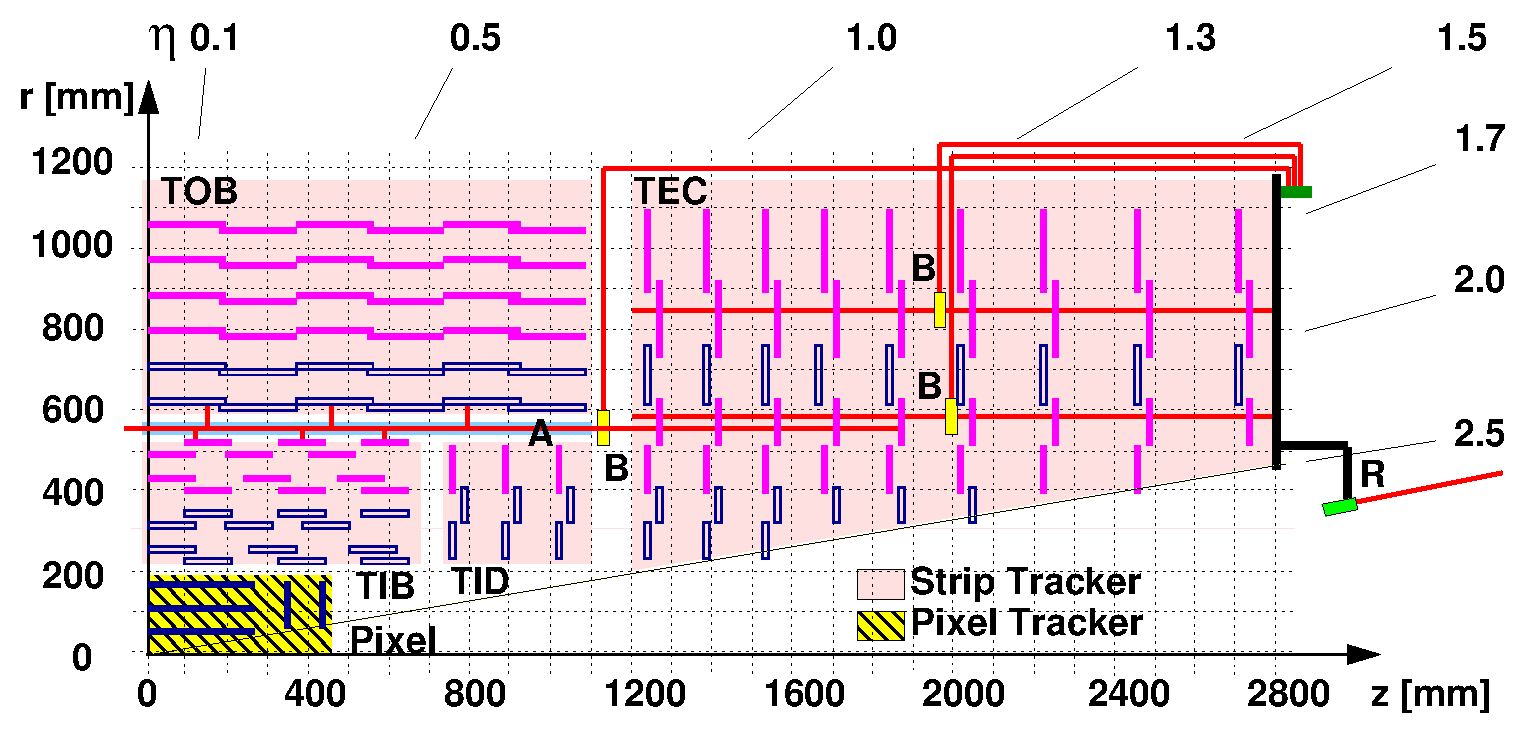
\includegraphics[width=.8\linewidth]{Experiment/figures/TrackerSystemLAS.eps}
\caption[Geometry of the Tracker System]{Tracker cross-section (1/4 of the $z$ view). The pixel tracker is located at the innermost radii of the detector and is labeled in striped yellow. The strip tracker is composed of four regions: Tracker Inner Barrel (TIB), Tracker Outer Barrel (TOB), Tracker End Cap (TEC), and Tracker Inner Disks (TID). The blue pieces are double-sided modules while magenta are single-sided. In addition to the silicon sensors, an infrared laser alignment system is used to provide coarse calibration for the tracker.}
\label{fig:TrackerSystem}
\end{center}
\end{figure}

As particle flux will clearly be highest closest to the interaction point, the smallest elements must be placed to avoid oversaturating the electronics. Silicon pixels of size $100\times150$ $\mu\rm{m}^2$ are arranged in three cylindrical barrel layers at $r=$ 4.4 cm, 7.3 cm, and 10 cm each with a length of 53 cm plus two endcap annuli at $|z|=$ 34.5 and 46.5 cm with radius from $r=$ 6 cm to 15 cm. The pixels are arranged in modules with read-out chips (16 per module in the barrel, 2-10 per module in the endcap), each of which reads the output of an array of $52\times80$ pixels. The output and location of any active pixels are stored in a buffer, awaiting decision to be stored permanently or not from the Level-1 Trigger (see Sec.~\ref{sec:Triggers}).

Outside of the pixel layers, the particle flux will be lower. Tracker elements can be a bit larger without oversaturating, so silicon microstrips are used (minimum cell size of 10 cm $\times$ 80 $\mu$m for $20 < r < 55$ cm and 25 cm $\times$ 180 $\mu$m for $r>55$ cm). The strip tracker is divided into four regions, named to indicate their location in the tracker subsystem: Tracker Inner Barrel (TIB), Tracker Outer Barrel (TOB), Tracker End Cap (TEC), and Tracker Inner Disks (TID). The TIB consist of four layers covering $|z|<$ 65 cm while the TOB covers $|z|<$ 110 cm and is made of six layers. By the orientation and size of the components, the barrel has single-point $r-\phi$ resolution of 23-34 $\mu$m (35-52 $\mu$m) and $z$ resolution of 230 $\mu$m (530 $\mu$m) in the TIB (TOB). For the endcap region, the TID is made of three rings that fill the gap between the TIB and TOB while the TEC is made of 9 rings stretching from $120 < |z| < 280$ cm. As the radiation is even smaller in the outer regions of the tracker, the strips can be longer and thicker. In the TOB and six outermost layers of the TEC, the sensors are slightly thicker at 500 $\mu$m compared to the 320 $\mu$m thick sensors elsewhere. By associating multiple tracker hits, trajectories of charged particles can be constructed. The ultimate designed global track resolution can be seen for muons and pions (the lightest meson) in Fig.~\ref{fig:TrackEfficiency}.

\begin{figure}[htbp]
\begin{center}
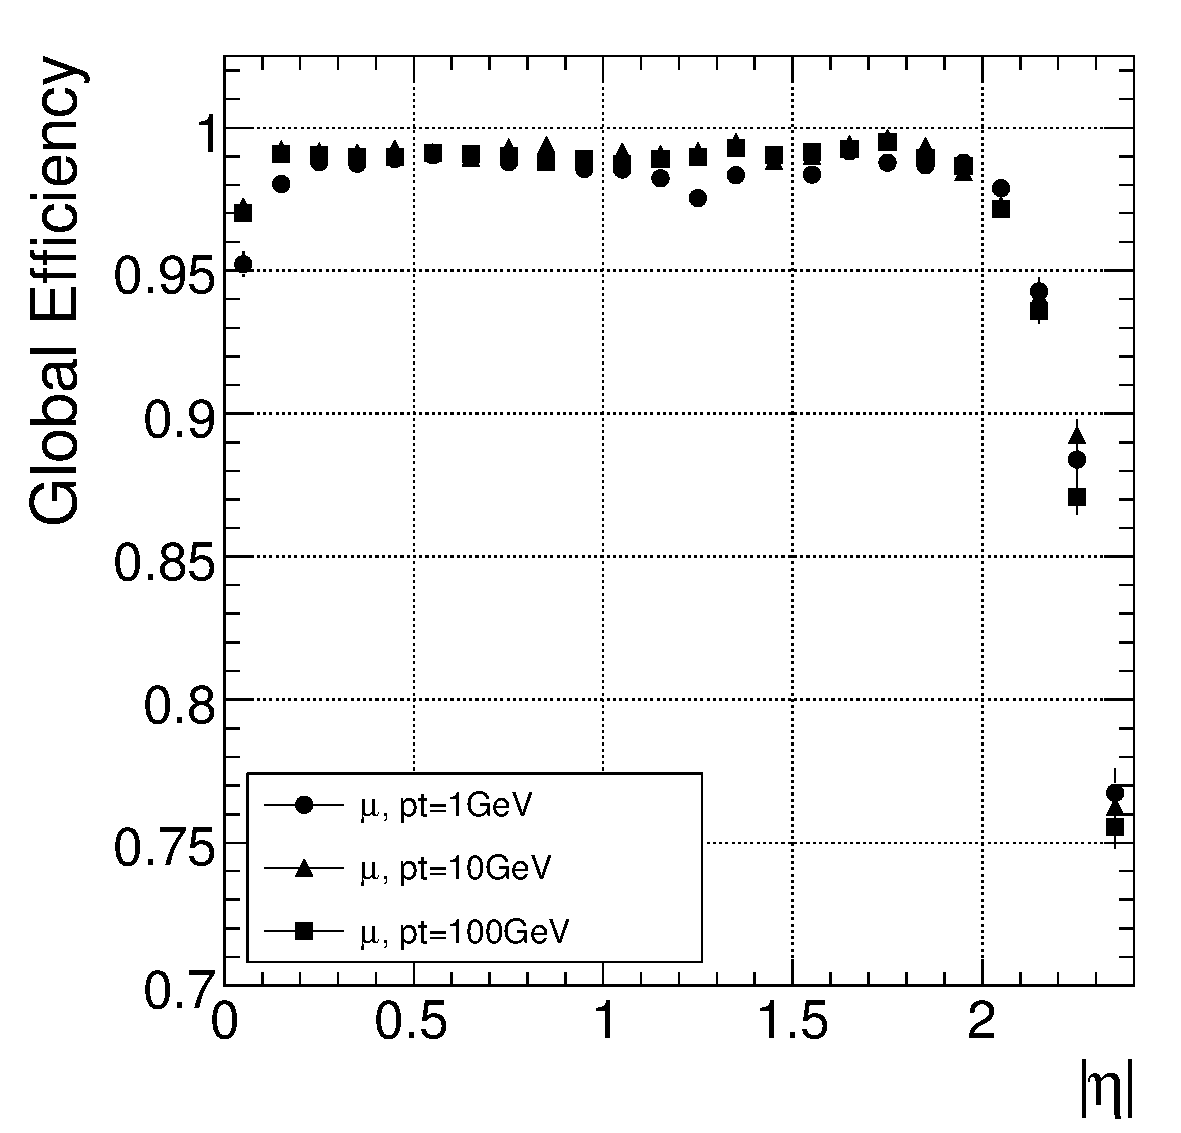
\includegraphics[width=.45\linewidth]{Experiment/figures/MuonTrackEfficiency.pdf}
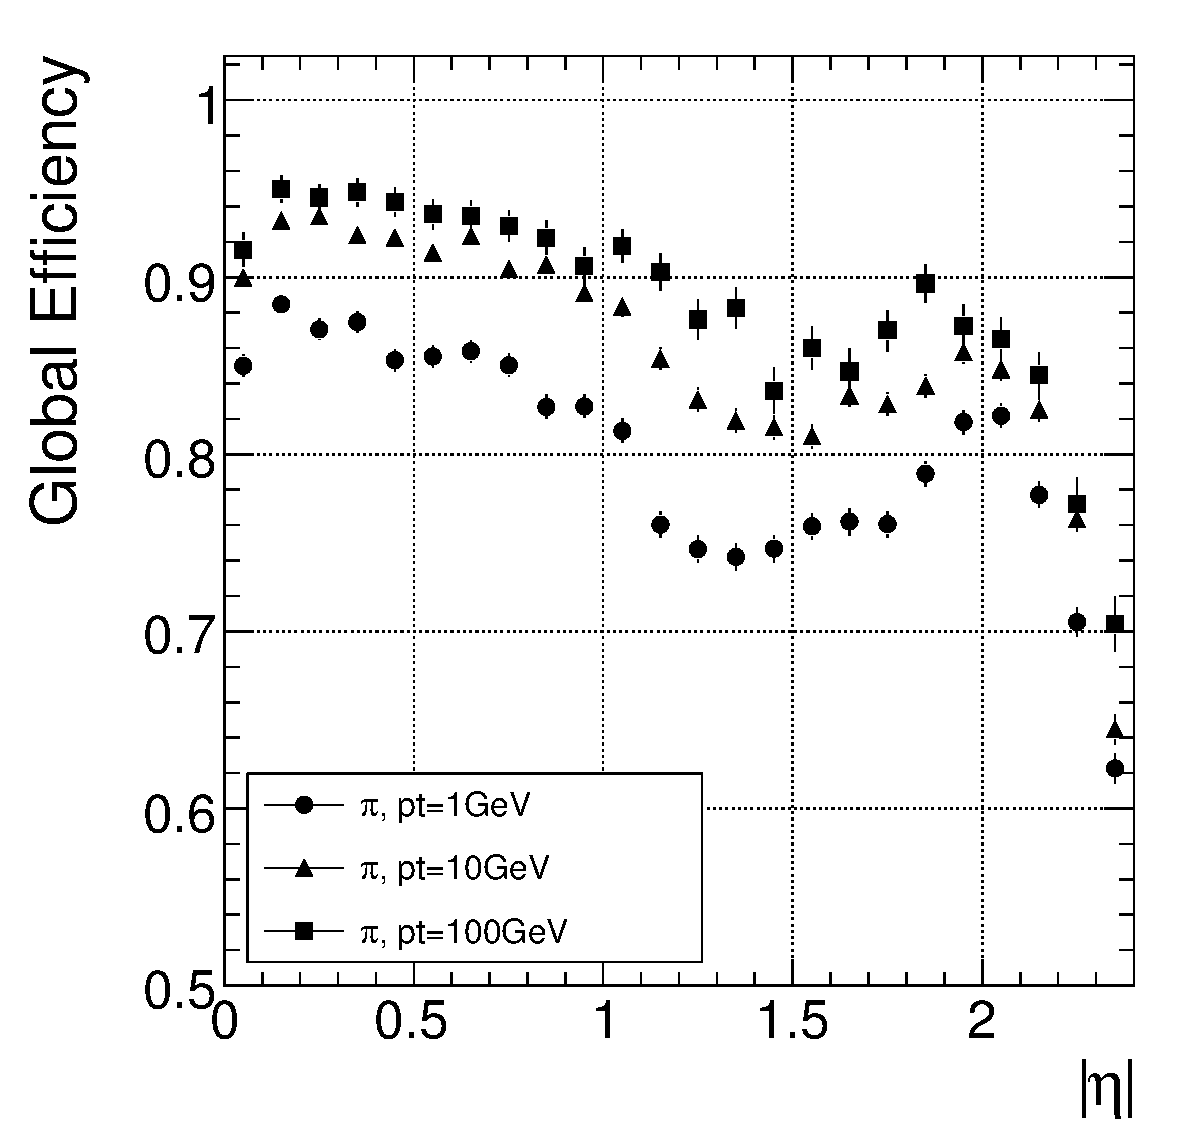
\includegraphics[width=.45\linewidth]{Experiment/figures/PionTrackEfficiency.pdf}
\caption[Global Track Reconstruction Efficiency at CMS]{Global track reconstruction efficiency of muons (left) and pions (right) for transverse momenta of 1, 10, and 100 $\rm{GeV}/c$. Overall efficiency decreases for smaller $p_T$ and near the edges of the detectable region.}
\label{fig:TrackEfficiency}
\end{center}
\end{figure}

As the tracker subsystem is the only one that can reconstruct vertices, great care is taken to affirm that the numerous pieces of the tracker are aligned to very high precision (ideally smaller than the single-point resolution, so $\lesssim10\mu\rm{m}$). After construction, a laser alignment system is used to calibrate the tracker, as well as other subsystems, to account for shifts in orientation. However, this method primarily accounts for large scale structure and not individual module misalignments. In sum, there are 9.6 million strips and 66 million silicon pixels spread across over 16000 modules, where the position and orientation of each must be tracked independently both before and during operation of CMS. The only way to account for all modules and get the desired detector position resolution is to use track-based alignment.

After measuring the positions of the various devices during construction and utilizing the laser alignment system, trajectories of known particles can be used to further the alignment. Since trajectories must be continuous, small misalignments of the modules will appear as discontinuities in the tracks. Looking for these discontinuities and measuring the pull of individual elements, the true orientation can be found.

In 2008, when the detector was fully constructed but the beam was not yet running, millions of cosmic muons were tracked through the detector. Computationally, to find the individual module corrections, it is equivalent to minimizing a matrix equation for $O(10^5)$ degrees of freedom, which is extraordinarily intensive. Nevertheless, using a combined method of algorithms to find global and local correlations, the positions of the modules were determined to an average precision of 3-4 $\mu$m in the barrel and 3-14 $\mu$m in the endcap in their respective most sensitive coordinate~\cite{Chatrchyan:2009sr}. Since environmental conditions of operation can cause deviations over time, similar alignment strategies are used by CMS during data collection.

\subsection{Particle Identification}
\label{sec:ParticleID}

During operation, when the proton beams collide, all of the subsystems work in tandem to identify different particles by what portions they interact with. For example, both muons and electrons will record hits in the tracker, but the muon will move through the muon system while electrons stop in the ECAL. Fig.~\ref{fig:CMSSliceWithTracks} shows a diagram with the expected interactions from a sample set of particles. In theory, it seems like this should be simple categorization: only electrons and photons interact with the ECAL, hadrons will interact with the HCAL, etc. Although it can be this simple, in practice, it is more nuanced. In one crossing, there are roughly 20-30 collisions and each can have multiple decay products which could deposit energies at similar locations; if a photon strikes the ECAL near an electron, how does CMS disentangle the two? Moreover, the lines between what particles interact with which subsystems aren't quite as rigid. Neutral pions will commonly decay to two photons and thus could mimic a photon in the ECAL, for example. Alternatively, an electromagnetic decay in the ECAL can leak into the HCAL. CMS accounts for these \textit{fake rates} and makes proper identifications by using the \textit{particle-flow algorithm}~\cite{ParticleFlowAlgo}. 

\begin{figure}[htbp]
\begin{center}
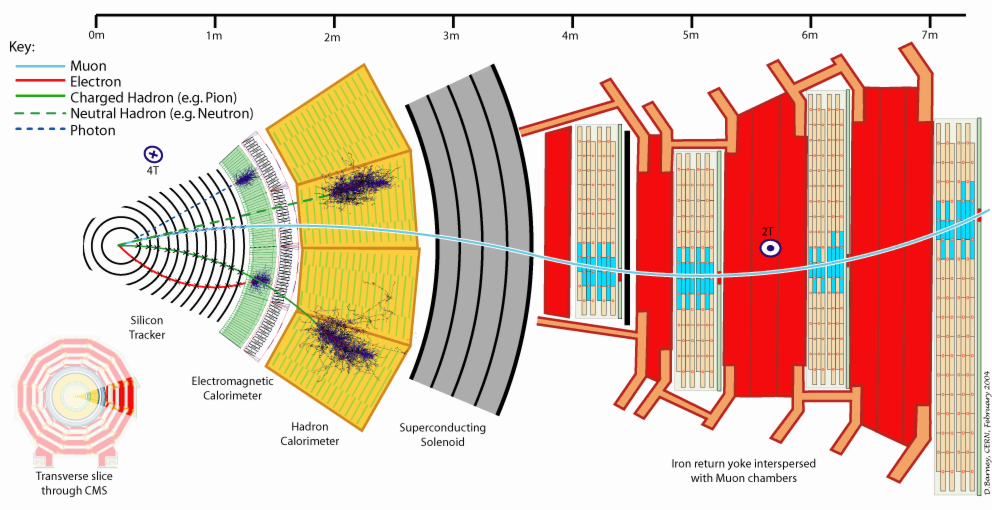
\includegraphics[width=.9\linewidth]{Experiment/figures/CMSSliceWithTracks.png}
\caption[Trajectories and Decays for Particle Identification in CMS]{Transverse slice of CMS with sample trajectories and decays from expected SM particles. Photons (dashed blue) and electrons will deposit their energy in the Electromagnetic Calorimeter, while both neutral (dashed green) and charged hadrons (green) deposit in the Hadronic Calorimeter. Muons (blue) will move through the muon system. All charged particles will interact with the tracker, leaving curved trajectories.}
\label{fig:CMSSliceWithTracks}
\end{center}
\end{figure}

Particle-flow links the output from the different subsystems to iteratively identify particles. For any charged particles, there will be tracks that should align with energy deposits in the calorimeters or muon system. Any hits in the calorimeters are clustered by looking for local maxima and associating nearby elements that are above threshold. In some cases, additional information can be used with the clustering. For example, in the ECAL, electrons will spread energy over a larger area of crystals that converted photons. These clusters (or trajectories in the muon system) are then matched to trajectories in the tracker system. Starting with a very tight cut between the two elements, matched particles and their associated hits in the subdetectors are removed from consideration and the algorithm repeats with a looser constraint.

This algorithm removes elements in a particular order\footnote{This is roughly in order of resolution for the expected particle, where each identification has little influence on successive identifications.}, starting with global muons, then electrons and photons, and finishing with jets. Once all particles are reconstructed, the missing transverse energy can be calculated. Finally, isolation can be used to indicate whether a given reconstructed particle is \textit{prompt}, meaning that it comes from an initial interaction. These reconstructed particles form the basic framework of all analyses at CMS. 

\subsection{Triggers}
\label{sec:Triggers}

As specified in Sec.~\ref{sec:LHC}, the intended number of collisions is on the order of 1 billion per second. However, even using state-of-the-art storage technology only about 100 events per second can be stored for later analysis, so nearly all of the collisions need to be rejected. Instead of arbitrarily taking data every hundredth of a second, a trigger system is designed so that only potentially interesting events can be captured. To determine what is interesting, data is temporarily stored and filtered by custom electronics. For the first trigger, Level-1, events are only accepted if they either have i) primitive objects from subsystems that pass $p_T$ or $E_T$ thresholds or ii) global $E_T$ or missing transverse energy ($E_T^{miss}$ or MET). The detector elements with fast time resolution, like the RPCs in the muon system (see Sec.~\ref{sec:MuonSystem}), define these primitive objects. Altogether, the Level-1 trigger procedure, including data transfer and decision making, is designed to be completed within 3.2 $\mu\rm{s}$ and reduces the rate of events to approximately 100 kHz.

After passing the Level-1 trigger, high level triggers (HLTs) apply additional processing to further reduce the throughput. Where the Level-1 triggers use primitive objects, HLT cuts on approximately reconstructed objects, applying thresholds for observables like $p_T$, relative isolation in the calorimeters and/or tracker, or $|\eta|$ of the particle. Although a primary purpose of the HLT cuts is to bring the event rate to 100 Hz, these cuts are tuned to be broadly applicable to different analyses, being maximally inclusive to the intended signal while minimizing backgrounds. Each analysis group can then select the data that pass the appropriate high level triggers to make a high precision measurement, exclude a theoretical model, or discover a new as-yet undetected particle.

\section{Summary}
\label{sec:expt_summary}

In 2008, after 25 years of construction, the LHC began operation. Within another two years, the combined energy of the beams reached 7 $\rm{TeV}$. In 2011, over 5 $\mathrm{fb}^{-1}$ was collected for 7 $\rm{TeV}$. After increasing the energy to 8 $\rm{TeV}$ in 2012, nearly another 20 $\mathrm{fb}^{-1}$ was collected. This was sufficient to confirm the existence of a Higgs-like boson, appearing to achieve one of the most elusive discoveries in particle physics. This chapter has reviewed the intricacies of the CMS detector itself, explaining the mechanism used to extract relevant information from the decays of trillions of high energy proton collisions. But how exactly was the new particle found in this mountain of data? How well can we measure its properties? Put bluntly, is this really the Higgs we've been looking for?
\chapter{Higgs Phenomenology at the LHC}
\label{sec:pheno}
\chaptermark{Higgs Phenomenology at the LHC}

\begin{center}
\begin{footnotesize}
{\it{``My drawing was not a picture of a hat. It was a picture of a boa constrictor digesting an elephant. Then, I drew the inside of the boa constrictor, so that the grown-ups could see it clearly. They always need to have things explained."}}\\
``Le Petit Prince", Antoine de Saint-Exup\'ery
\end{footnotesize}
\end{center}

\section{How to Find a Higgs at LHC}
\label{sec:LHCHiggs}

Just as with any other unstable particle in the Standard Model, when the LHC reaches a sufficient energy, the Higgs should be produced and then decay. Prior to discovery, it was known that if a SM Higgs boson existed, its production and decay must obey certain characteristics. By close examination of the decay products in CMS, we can pull back the curtain to see if a Higgs is hiding in one of these decay channels and if it matches the predictions of the Standard Model.

\subsection{An Interlude on Feynman Diagrams}
\label{sec:FeynDiagrams}

Before moving to specifics on how the Higgs is produced and decays at the LHC, we must diverge briefly to discuss production and decay more generally. Up to this point, we have been describing interactions in broad strokes, without delving into explicit mathematics. For the most part, we can continue without evaluating every integral and exponent, but these calculations still impact any analysis so we must find a way to encode these details. Fortunately, such a framework exists to represent the complicated mathematics behind the interactions of the Standard Model: \textit{Feynman Diagrams}. (Fig.~\ref{fig:FeynExample})

\begin{figure}[htbp]
\begin{center}
\unitlength=1mm
\begin{fmffile}{Phenomenology/figures/ComptonScattering}
\begin{fmfgraph*}(40,40)
  \fmfleft{i1,i2} \fmfright{sp1,sp2}
  \fmf{fermion,label=$e^+$}{i1,v1,sp1}
  \fmf{fermion,label=$e^+$}{i2,v2,sp2}
  \fmf{photon,label=$\gamma$}{v1,v2}
\end{fmfgraph*}
\end{fmffile}
\caption[Compton Scattering as an Example Feynman Diagram]{Compton Scattering as an example Feynman Diagram. With time going forward from left to right, two electrons approach each other, scatter via exchange of a photon, then move apart.}
\label{fig:FeynExample}
\end{center}
\end{figure}


In the most naive terms, particle physics measurements can be reduced to one goal: given initial particle states, what is the probability of producing a particular set of final particle states? As previously discussed in Sec.~\ref{sec:LHC}, the cross section of an event quantifies this probability, but it must be calculated somehow. In quantum field theories, the mathematical operation to convert incoming particle states to outgoing states via allowed operations of the model is the \textit{S-matrix}. Embedded in this matrix is the \textit{scattering matrix element} (commonly shortened to matrix element), $\mathcal{M}$, which encodes the full details of the interactions of a particular theory. The heuristic approach used to calculate the matrix element comes from summing the evaluations of all possible fully-connected\footnote{To be fully-connected, all incoming and outgoing particles must interact. In the calculation, these diagrams must also be amputated: self-interactions for a single particle do not, by definition, interact with the other particles and thus any diagrams with these elements do not contribute.} Feynman diagrams. Finally, the cross section is dependent upon the modulus squared\footnote{In general, a matrix element can be complex. As with other quantities in quantum mechanics, the modulus squared of an amplitude (e.g. the amplitude multiplied by its complex conjugate) will lead to measurable quantities. This also allows for the possibility of interference between different amplitudes.} matrix element which can be evaluated from the Feynman diagrams according to the rules of the interactions in the Lagrangian\footnote{This is a beautiful and very nuanced result where, for the sake of brevity, all of the mathematical rigor has been swept under the rug. A more complete explanation can be found in Part I of Peskin and Schroeder's \textit{An Introduction to Quantum Field Theory}.}. 

In practice, finding the matrix element is a two-fold problem. First, one needs to write down every possible contributing diagram. Each diagram must be then evaluated using the Feynman rules of that interaction; quantum electrodynamics (QED, pertaining to electromagnetism) has one set of rules while quantum chromodynamics (QCD, pertaining to the strong force) has another. Typically, just finding every contributing process this involves an infinite set of diagrams, however it can be simplified by categorizing diagrams by their complexity.

The simplest diagrams, called \textit{tree-level} or \textit{leading order} (LO) diagrams, contain no loops or extra corrections. Consider the diagrams where both the initial and final state is an electron-positron pair. Since diagrams without interactions don't contribute, the only leading order diagrams are found in Fig.~\ref{fig:Bhabha}. The strongest rationale for this categorization is implied by the term leading order: tree-level diagrams usually make up the highest order of magnitude term in the calculation and thus can be good approximations of the full result. Diagrams with one-loop or one radiative correction are considered \textit{next-to-leading order} (NLO), two loops are \textit{next-to-next-to-leading order} (NNLO) and so on.

\begin{figure}
\begin{center}
\unitlength=1mm
\subfloat{
\begin{fmffile}{Phenomenology/figures/ElectronPositronScattering}
\begin{fmfgraph*}(40,40)
  \fmfleft{i1,i2} \fmfright{sp1,sp2}
  \fmf{fermion,label=$e^-$}{i1,v1,sp1}
  \fmf{fermion,label=$e^+$}{i2,v2,sp2}
  \fmf{photon,label=$\gamma$}{v1,v2}
\end{fmfgraph*}
\end{fmffile}
}
\subfloat{
\begin{fmffile}{Phenomenology/figures/ElectronPositronAnnihilation}
\begin{fmfgraph*}(40,40)
  \fmfleft{i1,i2} \fmfright{sp1,sp2}
  \fmf{fermion,label=$e^-$}{i1,v1}
  \fmf{fermion,label=$e^+$}{i2,v1}
  \fmf{fermion,label=$e^-$}{v2,sp1}
  \fmf{fermion,label=$e^+$}{v2,sp2}
  \fmf{photon,label=$\gamma$}{v1,v2}
\end{fmfgraph*}
\end{fmffile}
}
\end{center}
\caption[Feynman Diagrams of Bhabha Scattering]{Bhabha Scattering: an electron and positron scatter via exchange of a photon (left) and an electron-positron pair annihilate to a photon then pair produce back to an electron-positron pair (right). When looking at the probability of getting an electron-positron pair from an initial electron-positron pair, these are the leading order diagrams.}
\label{fig:Bhabha}
\end{figure}

For analyses at the LHC, this framework of Feynman diagrams underlies all levels of theoretical prediction: how a new particle could be produced, determining the most likely methods of decay, or simulating any showering or hadronization in the detector. To understand what particles should be observed from a particular process, specialized software called \textit{Monte Carlo generators} (MC) are used to produce the kinematics of expected events. This software is used to generate both background and signal samples by using the Monte Carlo method~\cite{} to populate kinematic distributions as determined from Feynman diagrams. Given the overall complexity of the decay chains at CMS, the simulation can be compartmentalized into different generators suited towards certain tasks (e.g. generation and initial decay of the Higgs, showering and hadronization, interactions with the specific detector). Once these samples are finalized, backgrounds can be compared to data and statistically significant deviations can indicate areas of new physics.

\subsection{Higgs Production}
\label{sec:HiggsProduction}

Starting with the production of the Higgs at the LHC, a crucial factor comes from use of protons in collisions. As mentioned in Sec.~\ref{sec:FundParticles}, protons are made up of a veritable sea of quarks and gluons. So when two protons collide, this is better thought of as a piece of one proton interacting with a piece of the other. Whether these pieces, called \textit{partons}, are quarks or gluons determine the allowed paths that can be taken to generate a given Feynman diagram. Unfortunately, as we only detect the decay products from an event, the initial state partons can only be determined probabilistically via the \textit{parton distribution function} (PDF). For example, events that use a small fraction of the total energy of the incident proton are much more likely to come from a lower energy gluon than the up or down valence quarks. Due to the theoretical complexity of QCD, these functions are only computed experimentally and can become a source of systematics in any analysis. Nevertheless, since the mass of the Higgs was predicted to be well below the total energy of the beam, the possible production mechanisms of the Standard Model Higgs are well understood.

\begin{figure}
\begin{center}
\unitlength=1mm
\subfloat{
\begin{fmffile}{Phenomenology/figures/ggFProduction}
\begin{fmfgraph*}(40,40)
  \fmfleft{i1,i2} \fmfright{o1}
  \fmf{gluon,label=$g$,l.d=10}{i1,v1} \fmf{gluon,label=$g$}{i2,v2}
  \fmf{fermion,label=$t$}{v1,v2}
  \fmf{fermion,label=$\bar{t}$}{v3,v1}
  \fmf{fermion,label=$t$,label.side=left}{v2,v3}
  \fmf{dashes,label=$H$}{v3,o1}
\end{fmfgraph*}
\end{fmffile}
}
\subfloat{
\begin{fmffile}{Phenomenology/figures/VBFProduction}
\begin{fmfgraph*}(40,40)
  \fmfleft{i1,i2}
  \fmfright{sp1,sp2,sp3}
  \fmf{fermion,label=$q_1$,label.side=left}{i1,v1}
  \fmf{fermion,label=$q_1'$,label.side=left}{v1,sp1}
  \fmf{fermion,label=$q_2$,label.side=left}{i2,v3}
  \fmf{fermion,label=$q_2'$,label.side=left}{v3,sp3}
  \fmffreeze
  \fmf{photon,label=$V$}{v1,v2}
  \fmf{photon,label=$V$}{v2,v3}
  \fmf{dashes,label=$H$}{v2,sp2}
\end{fmfgraph*}
\end{fmffile}
}

\subfloat{
\begin{fmffile}{Phenomenology/figures/VHProduction}
\begin{fmfgraph*}(40,40)
  \fmfleft{i1,i2} \fmfright{o1,o2}
  \fmf{fermion,label=$q$}{i1,v1} \fmf{fermion,label=$\bar{q}$}{i2,v1}
  \fmf{photon,label=$V^*$}{v1,v2}
  \fmf{photon,label=$V$}{v2,o1}
  \fmf{dashes,label=$H$}{v2,o2}
\end{fmfgraph*}
\end{fmffile}
}
\subfloat{
\begin{fmffile}{Phenomenology/figures/ttHProduction}
\begin{fmfgraph*}(40,40)
  \fmfleft{i1,i2}
  \fmfright{sp1,sp2,sp3}
  \fmf{gluon,label=$g$,l.d=10}{i1,v1}
  \fmf{fermion,label=$\bar{t}$,label.side=left}{sp1,v1}
  \fmf{gluon,label=$g$,l.d=10}{i2,v3}
  \fmf{fermion,label=$t$}{v3,sp3}
  \fmffreeze
  \fmf{fermion}{v1,v2}
  \fmf{fermion}{v2,v3}
  \fmffreeze
  \fmf{dashes,label=$H$}{v2,sp2}
\end{fmfgraph*}
\end{fmffile}
}
\end{center}
\caption[Higgs Production Mechanisms]{Most common production mechanisms for the Higgs boson at the LHC: gluon-gluon fusion (top left), vector boson fusion where $V=W,Z$ (top right), Higgs-strahlung where $V=W,Z$ (bottom left), associated production with $t\bar{t}$ (bottom right).}
\label{fig:HiggsProductionFeyn}
\end{figure}

There are four major production mechanisms for the Higgs at the LHC, see Fig.~\ref{fig:HiggsProductionFeyn}. Their contribution as a function of the mass of the Higgs is seen in Fig.~\ref{fig:HXSWGProduction}. \textit{Gluon-gluon fusion} (ggF) is the most likely production mechanism of the Higgs (87\% near 125 $\rm{GeV}$). Even though ggF requires a fermionic loop, gluons are the most likely partons from the colliding protons, so this method dominates. The effective coupling of the Higgs to gluons through this loop is proportional to the mass of the quark in the loop, so the top, being the most massive quark, is the most likely contributor. 

After gluon-gluon fusion, the Higgs is most likely (7\% near 125 $\rm{GeV}$) to be produced through \textit{vector boson fusion} (VBF). A quark from each proton radiates a vector boson (either the $W$ or $Z$, since photons are massless, they do not directly couple to the Higgs) which collide to make the Higgs. A crucial feature compared with gluon-gluon fusion is that there are two quarks inherent in the production which can become detectable jets. Due to gluon radiation, ggF can also have jets in the final decay products, but jets from VBF production have substantially different kinematics, aiding in their discrimination in any Higgs analysis (see Sec.~\ref{sec:VBFVertex}).

As the Higgs mass is restricted to be above either $m_W$ or $m_Z$, it is energetically unfavorable for a $W$ or $Z$ to decay to the Higgs. However, quantum field theories allow for internal lines in Feynman diagrams (propagators) to become virtual and move \textit{off-shell}\footnote{The shell referred to in on- and off-shell is the mass shell. Classical particles obey the energy-momentum relation $E^2=p^2c^2 + m^2c^4$ where $E$ is the particle's energy, $p$ is its momentum, and $m$ is its mass. Virtual particles are not bound by this relation.}. Where \textit{on-shell} particles (with a mass near the bare mass, i.e $m_W$ and $m_Z$ for the $W$ and $Z$ respectively) can be directly observed, off-shell particles are forced to decay by the uncertainty principle. Thus, an off-shell $W^*$ or $Z^*$ can radiate a Higgs to return to an on-shell $W$ (WH) or $Z$ (ZH). This process (3\% for WH, 2\% for ZH at 125 $\rm{GeV}$) is called \textit{Higgs-strahlung} as it is reminiscent of electrons radiating photons in bremsstrahlung. Unsurprisingly, as the Higgs' mass increases, the $W$ or $Z$ must be further off-shell, so this process will contribute less to the overall cross section.

The last major production mechanism is \textit{associated production with heavy quarks}. Strictly speaking, this can include production of the Higgs with any pair of heavy quarks, but $t\bar{t}+H$ (ttH) is the only one included in the analyses of this thesis. The expected number of ttH events in CMS is quite small and other heavy quark combinations are even smaller.

\begin{figure}[htbp]
\begin{center}
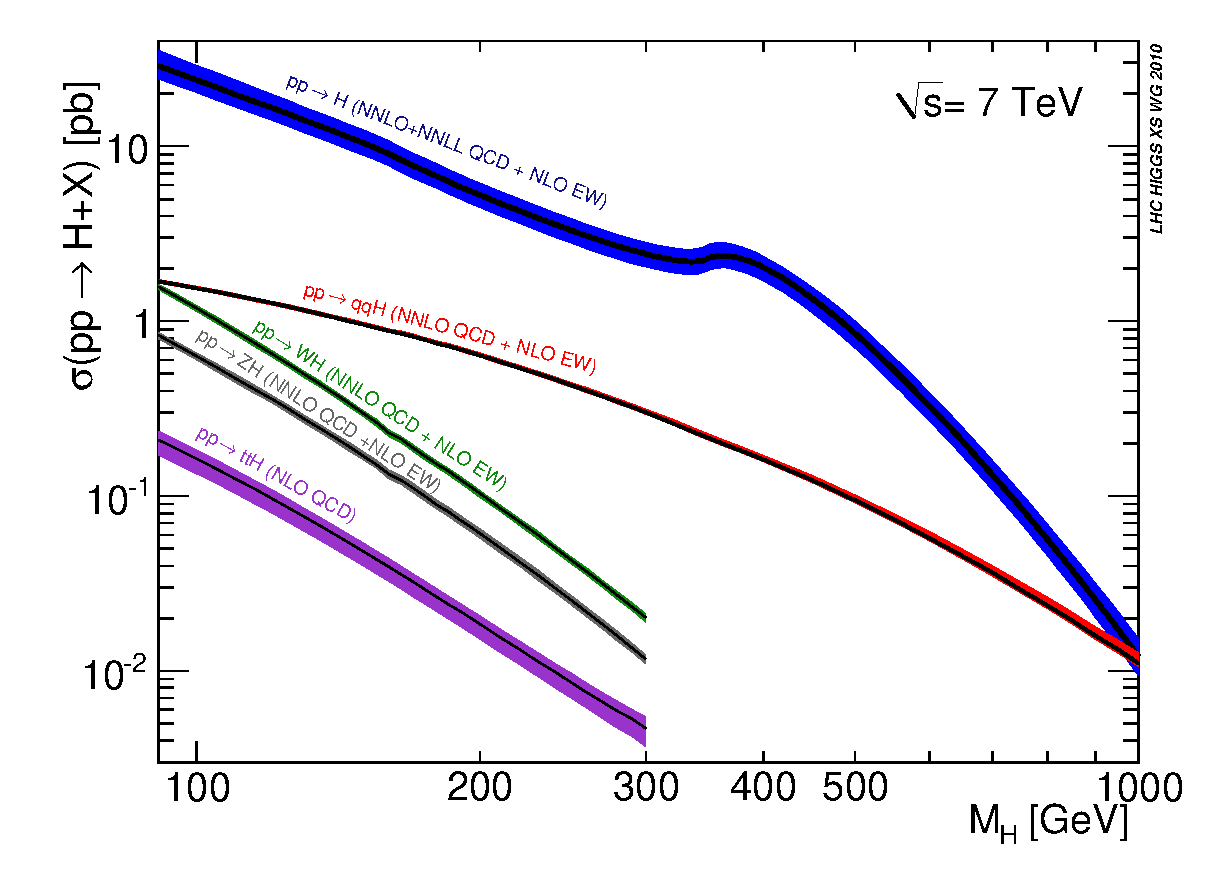
\includegraphics[width=.45\linewidth]{Phenomenology/figures/Higgs_XS_7TeV}
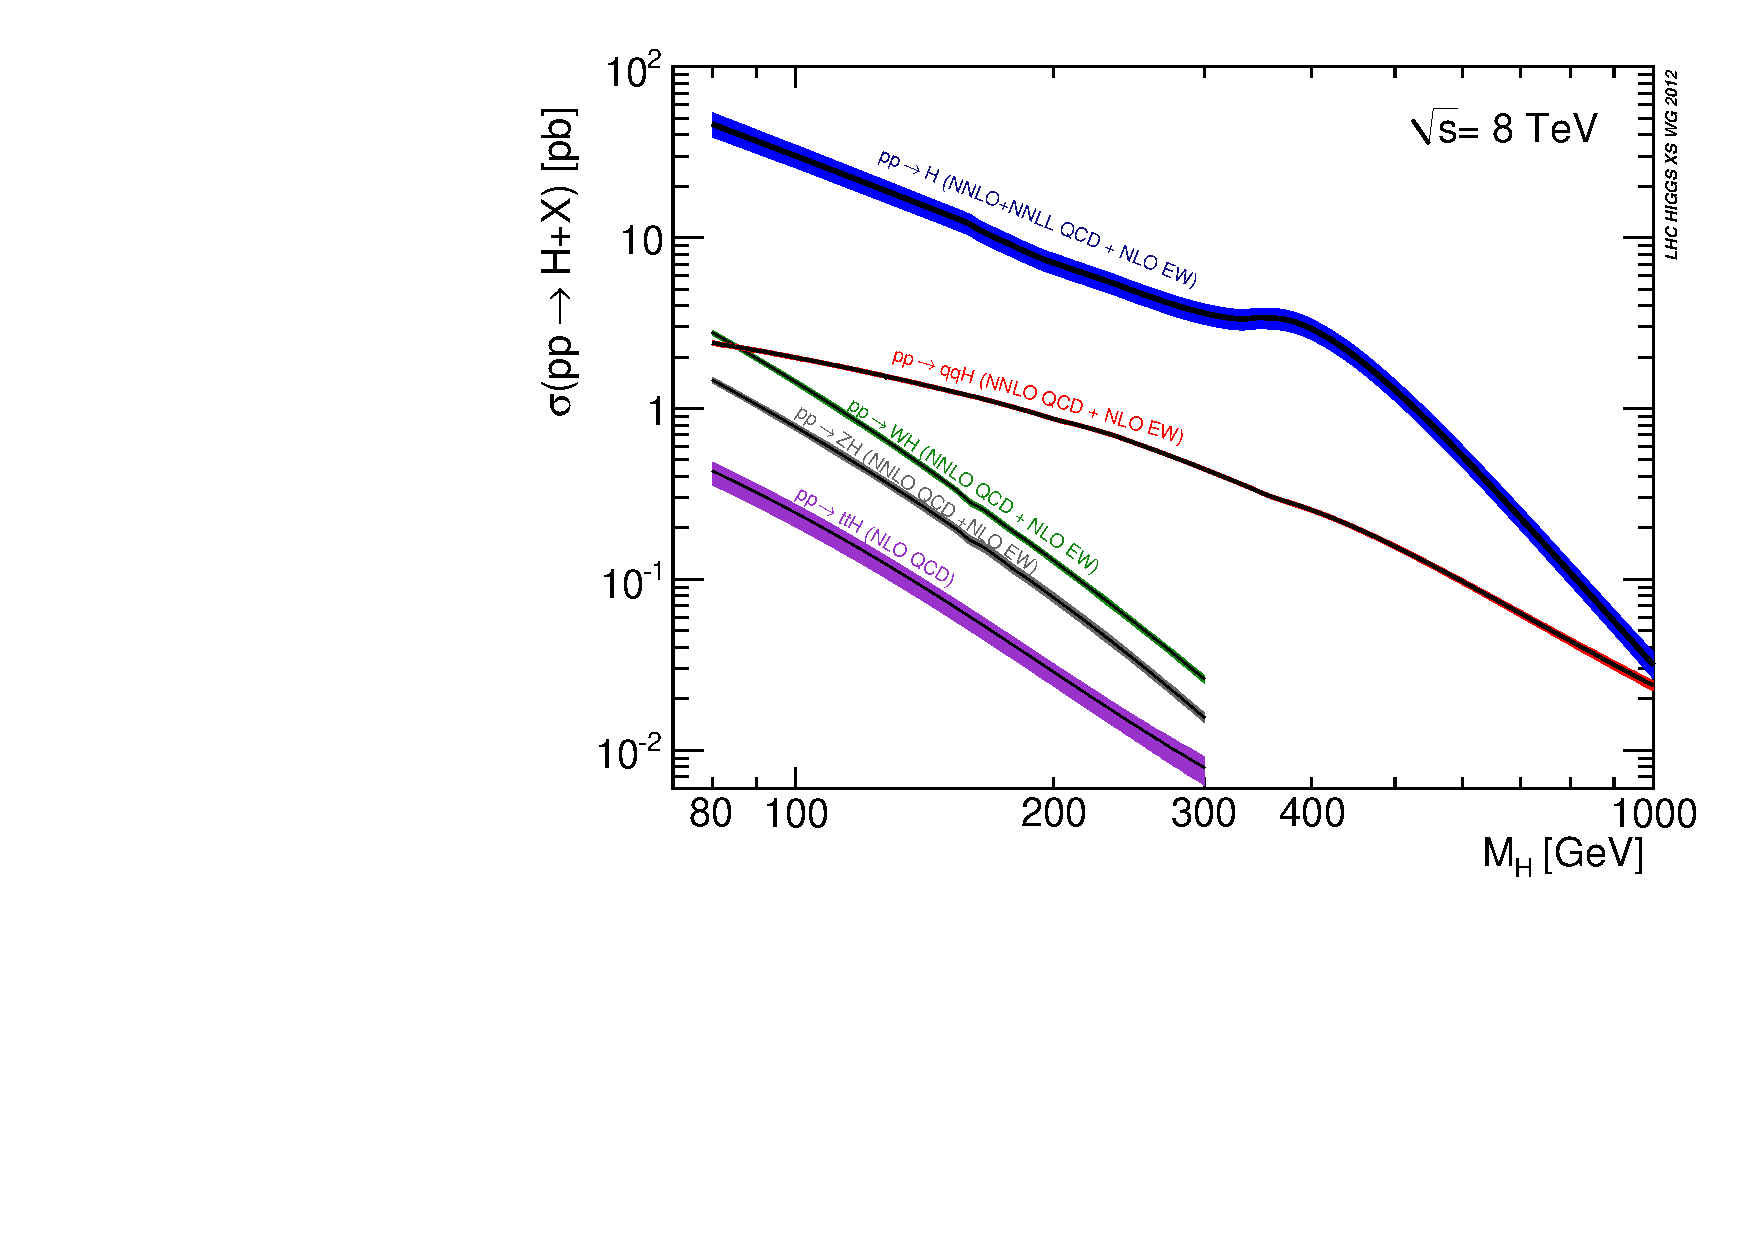
\includegraphics[width=.45\linewidth]{Phenomenology/figures/Higgs_XS_8TeV_lx.pdf}
\caption[Standard Model Production Mechanism of the Higgs at the LHC as a Function of the Higgs' Mass]{SM Cross sections of the different production mechanisms of the Higgs as a function of $m_H$ in the LHC for $\sqrt{s}=$ 7 $\rm{TeV}$ (left) and 8 $\rm{TeV}$ (right) with uncertainty bands~\cite{HXSWG}. Gluon-gluon fusion (blue) dominates until $m_H \approx 1$ $\rm{TeV}$, where vector boson fusion (red) becomes dominant. WH (green), ZH (grey), and ttH (purple) become energetically unfavorable for higher values of $m_H$.}
\label{fig:HXSWGProduction}
\end{center}
\end{figure}

\subsection{Higgs Decay}
\label{sec:HiggsDecay}

Once the Higgs is produced at LHC, it can decay through any of the allowed channels. Since the SM Higgs couples to both fermions and bosons according to their mass, it can decay at leading order to any pair of massive particles and to massless particles at next-to-leading order via one loop. However, what pair is most favorable depends on the mass of the Higgs, quantified as the \textit{branching ratio} as seen in the left plot of Fig.~\ref{fig:HXSWGDecay}. For $m_H\lesssim2\times m_W$, the Higgs is most likely to decay to a $b\bar{b}$ pair because the $m_b = 4.2 \rm{GeV} \ll m_H$ so the $b$-quarks will be on-shell. For $2\times m_t \gtrsim m_H \gtrsim 2\times m_Z$, $H\rightarrow WW$ and $H\rightarrow ZZ$ can decay to two on-shell bosons, so they become the dominant decays. Lastly, for the highest mass ranges, $m_H \gtrsim 2\times m_t$, the Higgs can also decay to two on-shell top-quarks, so $H\rightarrow t\bar{t}$ becomes much more prevalent. It does not dominate bosonic decay, however, because the fermionic coupling is proportional to the mass of the fermion whereas bosonic coupling is proportional to the square of the mass of the boson.

\begin{figure}[htbp]
\begin{center}
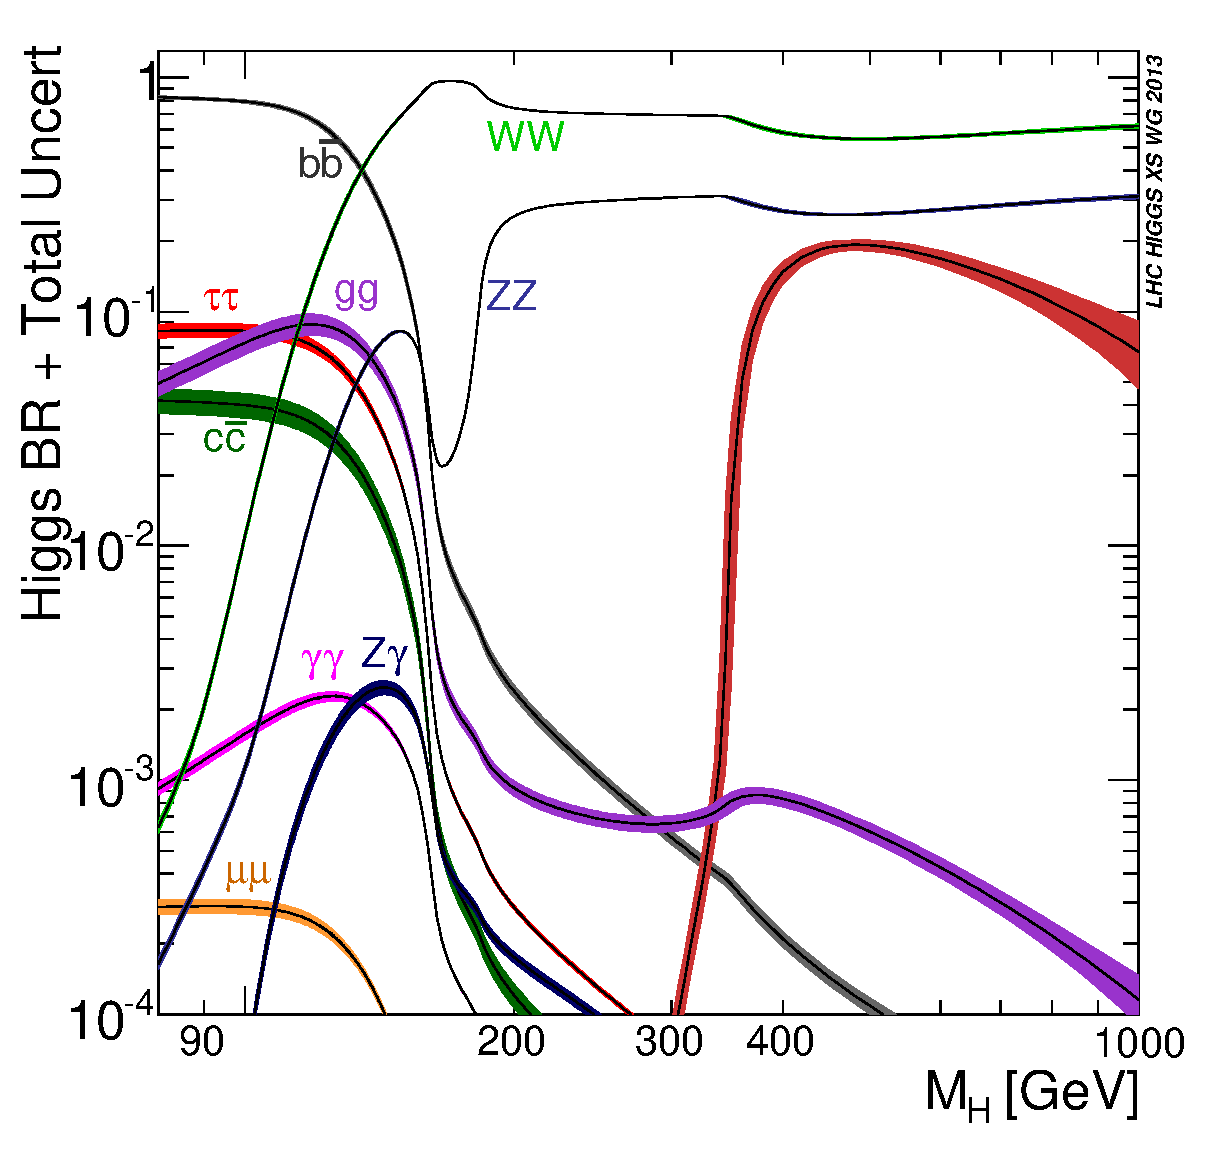
\includegraphics[width=.45\linewidth]{Phenomenology/figures/Higgs_BR}
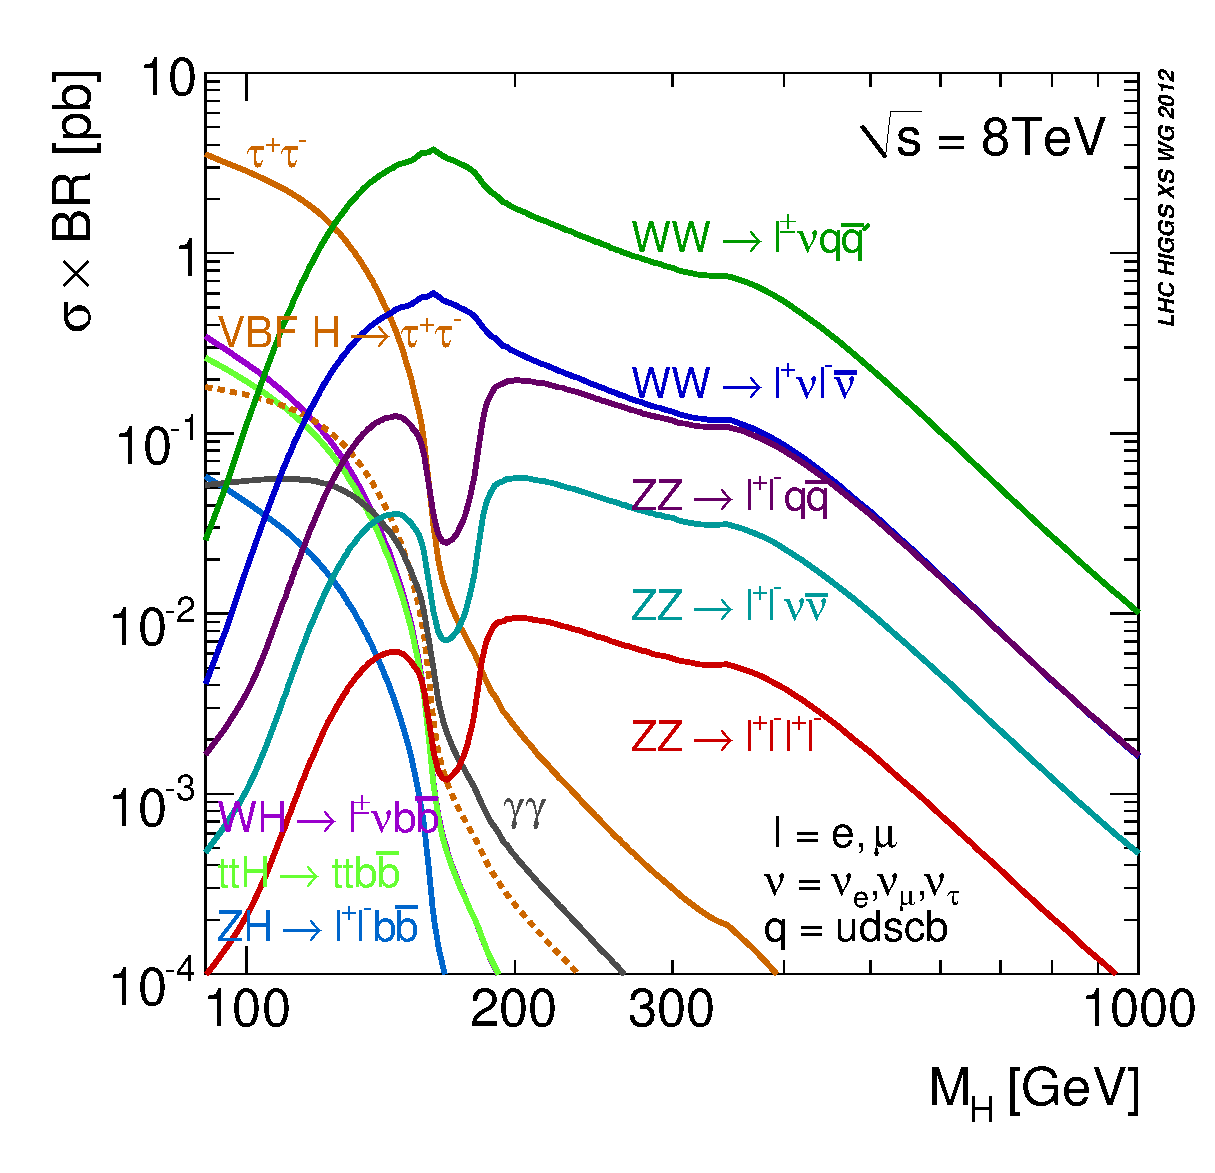
\includegraphics[width=.45\linewidth]{Phenomenology/figures/XSBR_8TeV_SM_HM}
\caption[Standard Model Decay Branching Ratios for the Higgs at the LHC as a Function of the Higgs' Mass]{SM Branching Ratio of the Higgs through different decays with uncertainty bands (left). SM cross sections times branching ratio at the LHC for $\sqrt{s}=$ 8 $\rm{TeV}$ (right).~\cite{HXSWG}}
\label{fig:HXSWGDecay}
\end{center}
\end{figure}

In CMS, the different analyses of the Higgs are grouped by the final state. For $H\rightarrow \gamma\gamma$ or $H\rightarrow\tau^+\tau^-$, the direct decays of the Higgs are final state. For $H\rightarrow WW$ or $H\rightarrow ZZ$, how the $W$ or $Z$ decays plays a large role in what backgrounds are applicable, so the analyses are further grouped by the decays of the bosons (e.g. $H\rightarrow W^+W^- \rightarrow (l^+\nu)(l^-\nu)$ or $H\rightarrow ZZ \rightarrow (l^+l^-)(q\bar{q})$). In any given Higgs analysis, there are two competing interests: i) maximize the number of expected Higgs events while ii) minimizing the background to increase the overall significance of any signal. The cross sections of the given decay channel as a function of the Higgs mass are displayed in the right plot of Fig.~\ref{fig:HXSWGDecay}.

For most of the valid mass range, $WW\rightarrow l^{\pm}\nu q\bar{q}$ should have the highest number of expected Higgs events. But, any state with quarks in the decay will need to compete with a large background from QCD processes, plus the momentum resolution for jets is not as good as leptons. Furthermore, any decay with neutrinos involves missing energy, meaning that the full kinematics of the $H\rightarrow ZZ\rightarrow 4l$ decay cannot be uniquely determined. For this reason, $ZZ\rightarrow 4l$ is called the ``golden" channel. The full kinematics of the Higgs decay can be accounted for and, using proper cuts, the energy can be measured precisely with comparatively small backgrounds. Although the expected number of Higgs events in this channel will be small, the relative purity makes it ideal for discovery and property measurements of a Higgs boson. 

\section{Studying the $HVV$ Vertex}
\label{sec:HVVVertex}

Roughly speaking, there are two major vertices in the leading order contributions to Higgs production and decay\footnote{By the Feynman rules of the Standard Model, there are a total of five vertices with the Higgs: one Higgs boson and two fermions, one Higgs boson and two bosons, two Higgs bosons and two bosons, three Higgs bosons, and four Higgs bosons. The latter three are all subdominant, and thus beyond the direct scope of this thesis.}: Higgs coupling to two fermions (Hff) or to two bosons (HVV). Of the major production mechanisms from Sec.~\ref{sec:HiggsProduction}, ggF and ttH fall into the former category while VBF and VH fall into the latter. For decay, the $H\rightarrow ZZ \rightarrow 4l$ channel, which we will use in Sec.~\ref{sec:discovery} and~\ref{sec:properties}, involves an HVV vertex. Understanding how this vertex acts in the Standard Model versus a BSM Higgs or background could improve the sensitivity and illuminate what properties of the Higgs could be measured.

\subsection{$H\rightarrow VV$}
\label{sec:HVVDecay}

In the Standard Model, the Higgs boson is a CP-even spin-0 particle. But, as mentioned in Sec.~\ref{sec:findingBSM}, a newly discovered particle could violate CP-symmetry or be spin-2 instead of spin-0: that is, an observed boson may not be the SM Higgs and instead give credence to a BSM theory. For a generic spin-0 resonance $X$ decaying to two spin-1 gauge bosons ($V=Z,$ $W,$ or $\gamma$), the scattering amplitude can be written as~\cite{Anderson:2013aa}:
\begin{equation}
  \mathcal{A}(X_{J=0} \rightarrow VV) = \frac{1}{v}\left(g_1m_V^2\epsilon_1^*\epsilon_2^*+g_2f_{\mu\nu}^{*(1)}f^{*(2),\mu\nu}+g_4f_{\mu\nu}^{*(1)}\tilde{f}^{*(2),\mu\nu}\right)
\label{eq:scalarAmp_gform}
\end{equation}
where $v$ is the vacuum expectation value\footnote{The vacuum expectation value is the average value of a parameter in the vacuum, which is non-zero for the Higgs and is plotted in Fig.~\ref{fig:HiggsPotential}. For the Higgs, this value is 246 $\rm{GeV}$.} (VEV) of the SM Higgs field, $g_i$ are the spin-0 couplings with momentum-dependent form factors, $m_V$ is the mass of the boson, $f_{\mu\nu}^{(i)}=\epsilon_i^\mu q_i^\nu - \epsilon_i^\nu q_i^\mu$ is the field strength tensor\footnote{The field strength tensor, $f^{(i)\mu\nu}$, and dual field strength tensor, $\tilde{f}^{*(i)}_{\mu\nu}$, are mathematical representations of the electromagnetic fields in the system.} where $q_i$ is the momentum and $\epsilon_i$ is the polarization vector\footnote{For vector bosons in Electroweak Theory, polarization vectors indicate the orientation of the spin compared to the four-momenta. For each polarization state, the angular distributions of the decay will be limited due to conservation of angular momentum.} of the $i^{th}$ gauge boson, while $\tilde{f}^{(i),\mu\nu}=\frac{1}{2}\epsilon_{\mu\nu\rho\sigma}f^{(i),\rho\sigma}$ is the dual field strength tensor.

In the Standard Model, the Higgs preserves CP-symmetry, which correspond to the $g_1$ and $g_2$ coupling terms. For $m_V \neq 0$, such as $H\rightarrow ZZ$ or $H\rightarrow WW$, $g_1=2i$ at tree-level and is the dominant term while $g_2$ can contribute via radiative corrections (about $10^{-2}$). Clearly, for $m_V=0$, as in $H\rightarrow\gamma\gamma$ or $H\rightarrow gg$, the first term will not contribute so $g_2$ is dominant. The $g_4$ term corresponds to a CP-odd component, where the Higgs would be a pseudoscalar if dominant. For the SM Higgs, $g_4$ is extremely small ($O(10^{-10})$) as it only appears at the three-loop level. When the total decay rate is measured independently, as in the case of the $H\rightarrow ZZ \rightarrow 4l$ channel, it is more convenient to use the effective fraction of events to a particular coupling defined as
\begin{equation}
f_{gi} = \frac{|g_i|^2\sigma_i}{|g_1|^2\sigma_1 + |g_2|^2\sigma_2 + |g_4|^2\sigma_4}
\label{eqn:fgi_eqn}
\end{equation}
where $\sigma_i$ is the cross section for the $H\rightarrow VV$ process where $g_i=1,g_{j\neq i}=0$. In general, the $g_i$ couplings can be complex and the phase can be found via $\phi_{gi}=\rm{arg}{(g_i/g_1)}$. Additional amplitudes have been calculated for a spin-1 or spin-2 resonance decaying to two gauge bosons in~\cite{}.

For the case when a discovered neutral boson appears to be Higgs-like, i.e. $g_1 \gg g_{2,4}$, the amplitude can be rewritten to emphasize measurements of anomalous couplings compared to the SM predictions. Following the formalism used in~\cite{,,}, the amplitude can be rewritten as
\begin{equation}
\begin{split}
\mathcal{A}(X_{J=0} \rightarrow VV) = \frac{1}{v}\left(\left[ a_{1}  - e^{i\phi_{\Lambda{Q}}} \frac{\left(q_{1} + q_{2}\right)^{2}}{\left(\Lambda_{Q}\right)^{2}} - e^{i\phi_{\Lambda{1}}} \frac{\left(q_{1}^2 + q_{2}^2\right)}{\left(\Lambda_{1}\right)^{2}}\right]m_{V}^2 \epsilon_{1}^*\epsilon_{2}^*   \right. \\
\left. \vphantom{\frac{\left(q_{1} + q_{2}\right)^{2}}{\left(\Lambda_{Q}\right)^{2}}} + a_{2}^{}  f_{\mu \nu}^{*(1)}f^{*(2),\mu\nu} 
+ a_{3}^{}   f^{*(1)}_{\mu \nu} {\tilde f}^{*(2),\mu\nu}\right)
\end{split}
\label{eq:scalarAmpl_wformfactors}
\end{equation}
where the momentum dependence in the $a_1$ term is explicitly defined. $\Lambda$ and $\Lambda_{Q}$ are the mass scales of BSM physics and $\phi_{\Lambda{1}}$ and $\phi_{\Lambda{Q}}$ are the phases of their respective terms. The $\Lambda_1$ term corresponds to new, not yet observed particles contributing to the $HVV$ vertex while $\Lambda_Q$ corresponds to the $H\rightarrow VV$ interaction having an overall momentum dependence such that there could be enhancement of the Higgs off-shell. Eqn.~(\ref{eqn:fgi_eqn}) can then be rewritten as the equations
\begin{align}
f_{ai} &= \frac{|a_i|^2\sigma_i}{|a_1|^2\sigma_1 + |a_2|^2\sigma_2 + |a_4|^2\sigma_4 + \sigma_{\Lambda_{1}}/(\Lambda_1)^4} \label{eqn:fai} \\
f_{\Lambda{1}} &= \frac{\sigma_{\Lambda_{1}}/(\Lambda_1)^4}{|a_1|^2\sigma_1 + |a_2|^2\sigma_2 + |a_4|^2\sigma_4 + \sigma_{\Lambda_{1}}/(\Lambda_1)^4} \label{eqn:fL1} \\
f_{\Lambda{Q}} &= \frac{\tilde{\sigma}_{\Lambda{Q}}/\left(\Lambda_Q\right)^4}{|a_1|^2\sigma_1 + \tilde{\sigma}_{\Lambda{Q}}/\left(\Lambda_Q\right)^4} \label{eqn:fLQ}
\end{align}
with $\sigma_i$ still corresponding to the respective cross sections for Eqns.~(\ref{eqn:fai}) and (\ref{eqn:fL1}), as it is in Eqn.~(\ref{eqn:fgi_eqn}). For Eqn.~(\ref{eqn:fLQ}), since $f_{\Lambda{Q}}$ can only be measured by comparing on-shell and off-shell, $\sigma_1$ now refers to the total on-shell cross section where $\tilde{\sigma}_{\Lambda{Q}}/\sigma_{1}=m_{H}^4$.

But how do these coupling ratios manifest in the observation of a resonance? In Eqn.~(\ref{eq:scalarAmpl_wformfactors}), there is clear dependence on the polarization vectors of the decay bosons. As detailed in~\cite{}, by conservation of angular momentum, the spin of the resonance restricts the allowed polarization vectors and thus the helicity amplitudes which can determine the angular distributions. In other words, for the SM Higgs, the spins of the decay gauge bosons are correlated which will have direct impact on the likely angular distributions of the final decay state. These expected distributions, derived directly from the matrix element, can be used to assign probabilities on an event-by-event basis to discriminate between the SM Higgs and a BSM model or between the SM Higgs and background.

For the generic $X\rightarrow VV \rightarrow 4f$ decay channel, in the rest frame of the resonance nine parameters are sufficient to fully characterize the kinematics: three masses ($m_X$, $m_{V1}$, $m_{V2}$) and six angles. Figure~\ref{fig:HVVAngles} shows five of these angles, with a final global rotation about the beam line making the sixth. The five angles in Fig.~\ref{fig:HVVAngles}, referred to collectively as $\vec{\Omega}$, are all influenced by the helicity distributions from the amplitude listed above. For $m_X > 2\times m_V$, both of the gauge bosons will be on-shell. But if $m_X < 2\times m_V$ then the only way this decay can be observed is if at least one of the gauge bosons are off-shell. The global rotation along with the spatial momentum of the resonance are not influenced by the spin-parity of the state, so they don't aid in discriminating between different models, although the spatial momentum assists in separation of production mechanisms.

\begin{figure}[htbp]
\begin{center}
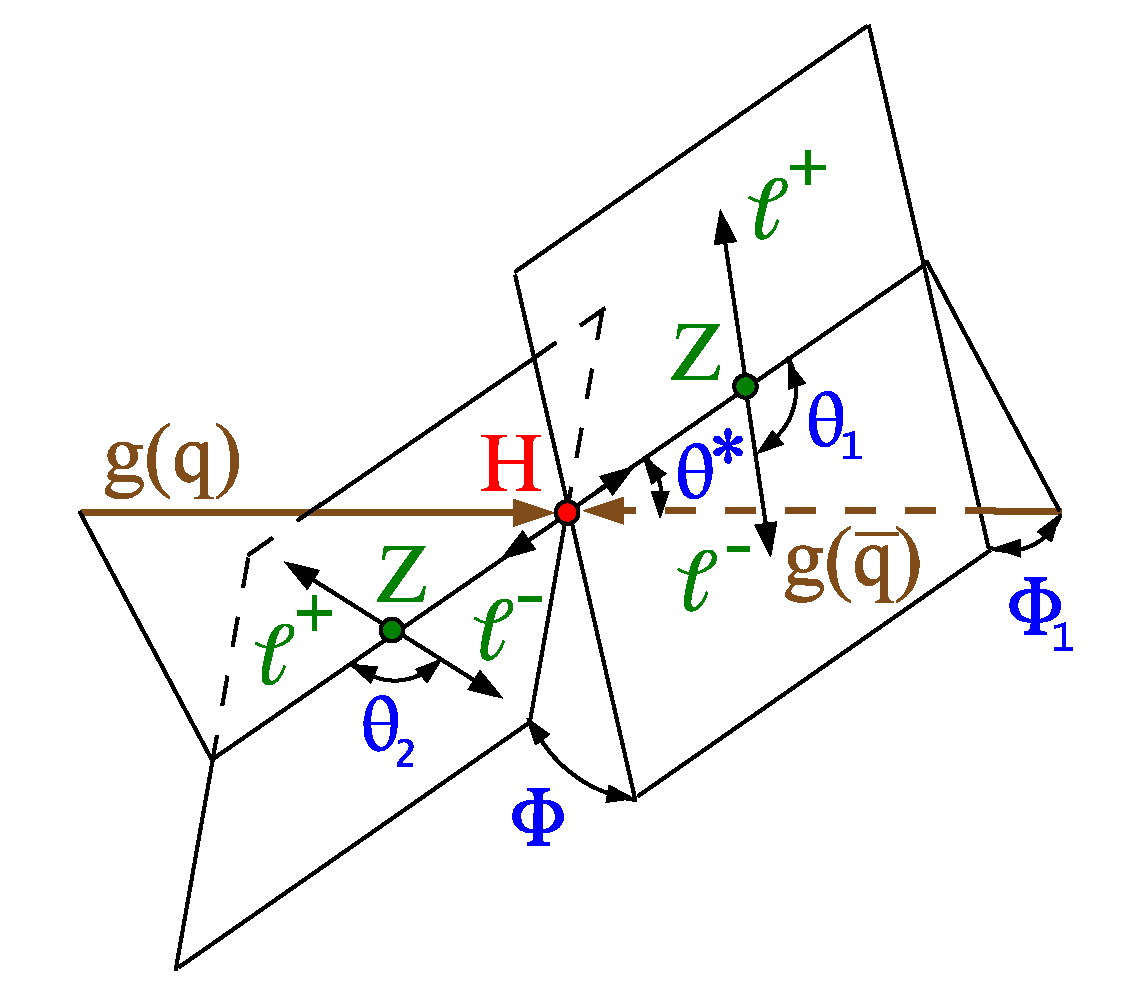
\includegraphics[width=.5\linewidth]{Phenomenology/figures/angles-HZZ4l.eps}
\caption[Definition of Angles in $H\rightarrow VV$ Decay]{Angles in the $H\rightarrow ZZ \rightarrow 4l$ decay as defined in the Higgs rest frame. Brown lines indicate incoming gluons or quarks along beam line. $\theta^*$ defines the angle from beam line to the decay line of the $Z$ bosons. $\Phi$ and $\Phi_1$ define the orientation of the planes for each $Z\rightarrow l^+l^-$ decay relative to the $H \rightarrow ZZ$ decay. $\theta_1$ and $\theta_2$ are the angles of the leptonic decay lines to the $Z_{1,2}$ momenta.}
\label{fig:HVVAngles}
\end{center}
\end{figure}

As stated in Sec.~\ref{sec:HiggsDecay}, the $ZZ\rightarrow 4l$ final state allows for precise and complete calculation of the decay kinematics, so this matrix element approach is ideal for Higgs searches of this final state. To discriminate background or alternative signals from the SM Higgs, there are two methods to analyze the three masses and five relevant angles of the decay kinematics on an event-by-event basis. A full 8D multidimensional fit could be used~\cite{}, but a very large number of events are required to properly populate the distributions, making it both computationally expensive and mostly inaccessible to decays with small yields. Alternatively, a single kinematic discriminant could be constructed where the information from the distributions is compounded into unified probabilities. This is the \textit{matrix element likelihood approach} (MELA)~\cite{,} which is used in CMS $ZZ\rightarrow 4l$ analyses.

Discriminants in MELA are built from probabilities, using the equation
\begin{equation}
\mathcal{D} = \frac{\mathcal{P}_{\rm{sig}}}{\mathcal{P}_{\rm{sig}} + \mathcal{P}_{\rm{bkg}}} = \left[1+ \frac{\mathcal{P}_{\rm{bkg}}(m_{4l};m_1,m_2,\vec{\Omega})}{\mathcal{P}_{\rm{sig}}(m_{4l};m_1,m_2,\vec{\Omega})}\right]^{-1}
\label{eq:MELADisc}
\end{equation}
where $\mathcal{P}_{\rm{bkg}}$ could refer to the probability from the dominant background in the analysis or an alternative signal hypothesis (e.g. a pseudoscalar Higgs) and $\mathcal{P}_{\rm{sig}}$ usually refers to the probability of the SM Higgs, though other signals could be used. Each probability ideally stems from an analytic matrix element, as is described in Eqn.~\ref{eq:scalarAmpl_wformfactors}, but when unavailable MC simulation can be used to populate the probability distributions. To account for this, the \textsc{JHU} generator (\textsc{JHUGen}) was written.

\textsc{JHUGen} is a dedicated MC generator, which full encodes the correlations and amplitudes of Eqn.~\ref{eq:scalarAmpl_wformfactors} as well as analogous amplitudes for spin-1 and spin-2 resonances. For $X\rightarrow VV$ decay, these matrix elements can be used in event generation or directly for building discriminants. Both properties will be utilized in the Higgs discovery (Sec.~\ref{sec:discovery}) and properties measurements (Sec.~\ref{sec:properties}). Comparisons of a few angular distributions from the analytic matrix element and the events from \textsc{JHUGen} are found in ~\cite{}.

\subsection{$VV \rightarrow H$}
\label{sec:VBFVertex}

\begin{figure}[htbp]
\begin{center}
\unitlength=1mm
\subfloat{
\begin{fmffile}{Phenomenology/figures/HVVVertex}
\begin{fmfgraph*}(40,40)
  \fmfleft{i1}
  \fmfright{sp1,sp2}
  \fmf{dashes,label=$H$}{i1,v0}
  \fmf{photon,label=$V$}{v0,sp2}
  \fmf{photon,label=$V$}{v0,sp1}
\end{fmfgraph*}
\end{fmffile}
}
\subfloat{
\begin{fmffile}{Phenomenology/figures/VVHVertex}
\begin{fmfgraph*}(40,40)
  \fmfleft{i1,i2}
  \fmfright{sp1}
  \fmf{photon,label=$V$}{i1,v0}
  \fmf{photon,label=$V$}{i2,v0}
  \fmf{dashes,label=$H$}{v0,sp1}
\end{fmfgraph*}
\end{fmffile}
}
\caption[Feynman Diagrams of the HVV vertex]{On left, the Higgs decays to two gauge bosons. On the right, two gauge bosons produce the Higgs. Any calculation of the amplitude of one vertex will be identical to the calculation of the time reversed vertex.}
\label{fig:HVVVertex}
\end{center}
\end{figure}

When looking at the $HVV$ vertex in Fig.~\ref{fig:HVVVertex}, it becomes obvious that $VV\rightarrow H$ is just a time reversal of the $H\rightarrow VV$ decay. The clear benefit is that, because the diagrams used to form the amplitude in Eqn.~\ref{eq:scalarAmp_gform} are identical, the end result is the same. The mathematical description provided by the matrix element approach in Sec.~\ref{sec:HVVDecay} applies to VBF production as well, with a few key differences:

\begin{description}
\item[Production v Decay Kinematics] \hfill \\
For VBF, the production kinematics are seen in Fig.~\ref{fig:VBFAngles}. For $H\rightarrow ZZ \rightarrow 4l$ decay, the kinematics of the decay can be fully defined using the three masses and five decay angles which can all be fully reconstructed. VBF is considerably more complicated as i) the direction and momentum fraction of the incoming partons are tied to the parton distribution function and ii) the production bosons transfer momentum from these incoming quarks.
\item[Universality of Decay Channel] \hfill \\
Although VBF is the subdominant production mechanism, it exists for every decay channel. Thus, measurements of the $HVV$ vertex can be combined across multiple analyses to improve overall performance.
\item[High Mass Sensitivity] \hfill \\
As the mass of the Higgs increases, VBF production becomes more and more likely. Any searches for high mass resonances should be tuned to emphasize VBF production.
\item[Cross Section Differences] \hfill \\
In Eqn.~(\ref{eqn:fai}), there is dependence on the anomalous cross section. Because of the large off-shell mass of $V^*$ in production, the ratio of anomalous cross section to SM cross section is considerably higher than in $H\rightarrow ZZ$ decay, allowing for higher precision with fewer events.
\end{description}

\begin{figure}[htbp]
\begin{center}
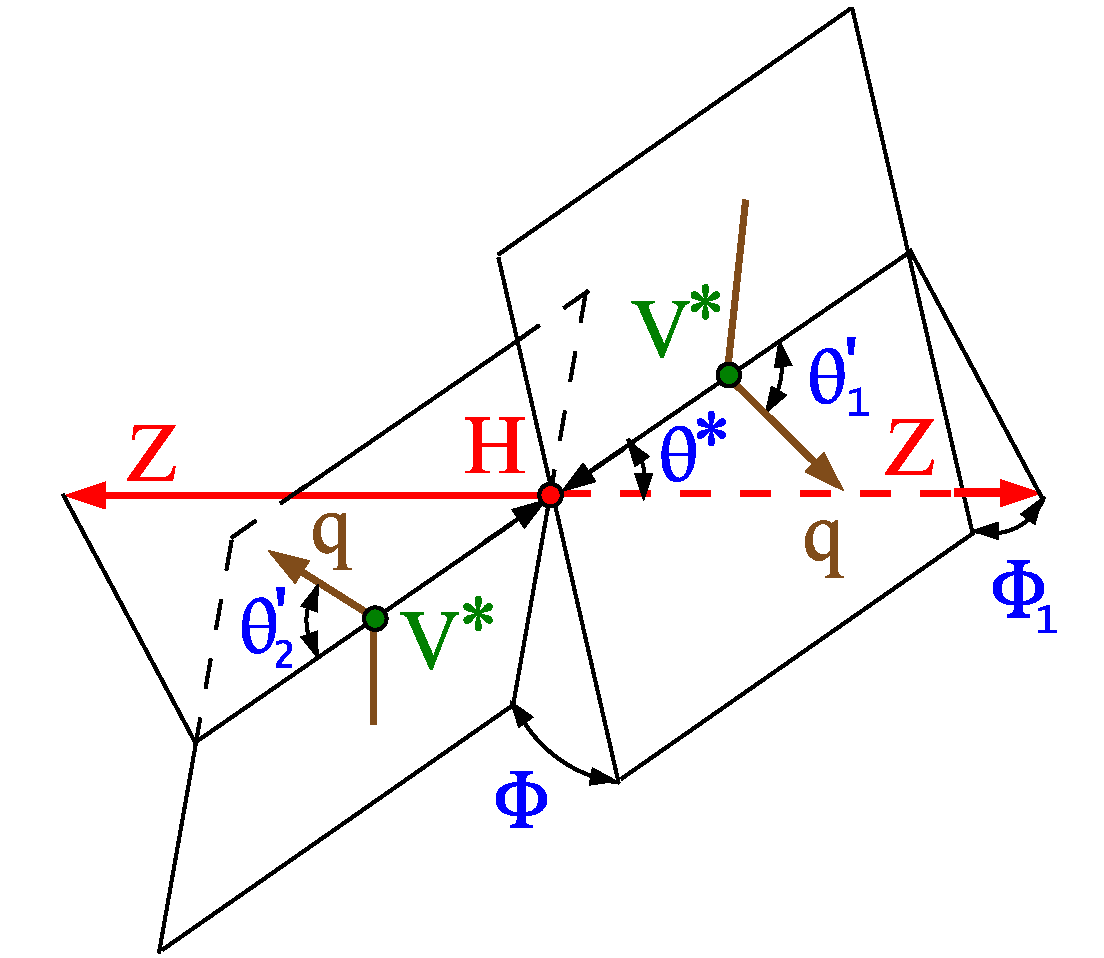
\includegraphics[width=.5\linewidth]{Phenomenology/figures/angles-HZZVBF_cms.pdf}
\caption[Definition of Angles in VBF Production]{Angles of VBF production in $H\rightarrow ZZ$. Compared to Fig.~\ref{fig:HVVAngles}, the angles mostly have similar definitions, but time reversed. The masses $m_{1,2}$ in decay are analogous to the  of the virtual $V^*$ bosons in production while $\theta_1^{'}$ and $\theta_2^{'}$ are analogous to $\theta_1$ and $\theta_2$, but the momentum lines for the incoming and outgoing quarks are not collinear.}
\label{fig:VBFAngles}
\end{center}
\end{figure}

Many BSM models predict multiple Higgs bosons of varying spin states. VBF production is crucial both to unambiguously discover new BSM particles across multiple decay channels and to use the $XVV$ vertex to measure the spin-parity state of any discovered resonance. Roughly speaking, although the full kinematics of the production are limited, the two jets that come from VBF production should have a wide forward-backward separation ($\Delta\eta$) and a large invariant mass of the dijet pair ($m_{JJ}$). Further correlations between these jets and the resonance can both illuminate its spin-parity and aid in the background separation. A numerical computation of the VBF matrix element is available in \textsc{JHUGen}, both for generation of events and calculation of probabilities for discriminants.

\subsection{$V^* \rightarrow VH$}
\label{sec:VHVertex}

Lastly, the $HVV$ vertex can be studied looking at Higgs-strahlung production. As with VBF in Sec.~\ref{sec:VBFVertex}, the mathematics of the generic amplitude in Eqn.~\ref{eq:scalarAmp_gform} are identical. In fact, if the final state $V$ boson decays to a jet pair, the decay products are also identical to VBF. However, where VBF expects a pair of strongly separated jets with a large invariant mass, the jet pair in VH production should have an invariant dijet mass, $m_{JJ}$, close to the on-shell mass of the $V$ boson. Modeling this with a gaussian\footnote{$m_{JJ}$ will be close to $m_V$, but resolution effects in the detector will smear out the true mass distribution.} about the expected $m_V$, the remaining kinematics can be used to build a probability. Although VH also depends on the parton distribution function, because the four-momentum of the VH pair can be well constructed and the incoming partons directly produce the virtual $V^*$, an analytic form of the matrix element is constructed and can be used in Higgs analyses.

\section{Summary}
\label{sec:pheno_summary}

Looking through the possible Higgs decay channels, analyzing in the $ZZ \rightarrow 4l$ decay channel is clearly a powerful method to search for the Higgs boson. By relying on the precise resolution for leptons in CMS, any $ZZ \rightarrow 4l$ event can be fully reconstructed. Then, these detailed kinematics can be used both in the search for the Higgs boson when comparing to backgrounds or in the measurement of its properties. In Sec.~\ref{sec:discovery}, we will use the techniques listed above to search for a Higgs boson. Then, in Sec.~\ref{sec:properties}, we will extract what the properties of this new boson are and whether it agrees with Standard Model expectations.

\chapter{Higgs Discovery in $ZZ\rightarrow4l$}
\label{sec:discovery}
\chaptermark{Discovery}

\begin{center}
\begin{footnotesize}
\textit{\textbf{Vladimir}: That passed the time.\\
\textbf{Estragon}: It would have passed in any case.\\
\textbf{Vladimir}: Yes, but not so rapidly.}\\
Samuel Beckett, ``Waiting for Godot"
\end{footnotesize}
\end{center}

\section{Backgrounds and Signals}

For MC we use

\section{Selection}

The triggers we use are

\section{Systematics}

As mentioned in Sec.

\section{Summary}
\label{sec:discovery_summary}
\chapter{Higgs Properties in $ZZ\rightarrow4l$}
\label{sec:properties}
\chaptermark{Properties}

\section{Higgs Width}
\label{sec:Width}

\section{Summary}
\label{sec:properties_summary}
\chapter{Conclusions and Outlook}
\label{sec:conclusions}
\chaptermark{Conclusions}

%\include{appendix}

%% REFERENCES

% if you use BIBTEX
\bibliographystyle{IEEEtran}
\bibliography{thesis}

\pagebreak
\begin{cv}{{\large Ian Anderson}\\
    {\normalsize Johns Hopkins University, 
      Department of Physics and Astronomy\\
      Email: ianderso@pha.jhu.edu
      \hfill Phone: {\mdseries 717-580-4187} 
    }
}
\fancyhead[RE,LO]{CURRICULUM VITAE}
\newlength{\oldcvlabelwidth}
\newlength{\oldcvlabelsep}

\setlength{\oldcvlabelwidth}{\cvlabelwidth}
\setlength{\oldcvlabelsep}{\cvlabelsep}

\setlength{\cvlabelwidth}{1em}

\begin{cvlist}{Education}
\item \emph{B.S., Physics}\\
Carnegie Mellon University, September 2005 - June 2009
\item \emph{M.A., Physics}\\
Johns Hopkins University, 2011
\item \emph{Ph.D., Physics}, expected Summer 2015\\
  Johns Hopkins University, September  2009 - present  
\end{cvlist}

\setlength{\cvlabelwidth}{0em}
\setlength{\cvlabelsep}{\labelsep}

%\begin{cvlist}{Awards \& Grants}
%\end{cvlist}
\begin{small}

\begin{cvlist}{Research Experience}
\item
\begin{itemize}\itemsep=0.25em
	\item Graduate Research, Johns Hopkins University, CMS Collaboration, 2011 - present
         	\begin{itemize}
		\item Off-shell study

	\end{itemize}
%	\item Senior Thesis, Princeton University, "Preliminary Measurements Towards Detailed State-to-State Collisional Population Transfer in Excited Atoms", Spring 2005
%	\item Summer Researcher, Princeton University - Summer 2004, Advisor: Michael Romalis; Summer 2002 \& 2003, Advisor: Daniel Marlow
%	\item Junior Paper, Princeton University, "Richness-Dependent Cluster Correlation Functions From SDSS Data", Spring 2004
%	\item Junior Paper, Princeton University, "CP Violation in Belle and the measurement of $\sin{2\phi_1}$ in $B^0~\rightarrow~\phi~K^0_s$", Fall 2003
%	\item Summer Researcher, Princeton University, Belle Collaboration, Advisor: Daniel Marlow, Summer 2002 \& 2003
\end{itemize}
\end{cvlist}

\begin{cvlist}{Teaching Experience}
\item
\begin{itemize}\itemsep=0.25em
	\item Teaching Assistant, General Physics I, Fall 2009 \& Spring 2011
	\item Teaching Assistant, General Physics II, Spring 2010 \& Spring 2012
	\item Teaching Assistant, Advanced Physics Lab, Spring 2013 \& Spring 2014
\end{itemize}
\end{cvlist}

\begin{cvlist}{Awards \& Grants}
\item
%	\item
%	NSF US LHC Graduate Student Support Award, 2009
%	\item 
%	URA Visiting Scholar, Fall 2009
\end{cvlist}

\begin{cvlist}{Presentations and Talks}
\item
%	\item
%	"Analysis of $Z \to l^+ l^-$ polarization at CMS", LHC students' poster session at next LHCC. Geneva, Switzerland, March 2011.	
%	\item
%	"Analysis of $Z \to l^+ l^-$ polarization at CMS", Recontres de Moriond, EW.  La Thuile, Italy, March 2011.
%	\item 
%	"Model-independent spin and coupling determination of Higgs-like resonances", Higgs Hunting Workshop.  Orsay, France, July 2010.	
%	\item
%	"Spin determination of single-produced resonances at the LHC", ICHEP 2010.  Paris, France, July 2010.	
%	\item
%	"Spin determination of single-produced resonances at the LHC", Fermilab Users' Meeting.  Batavia, IL, USA, June 2010.	
%	\item 
%	"Spin determination of single-produced resonances at the LHC", Pheno 2010 Symposium.  Madison, WI, USA, May 2010.
%	\item 
%	"Spin determination of single-produced resonances at the LHC", Northwestern University High Energy Physics Seminar.  Evanston, IL, USA, April 2010.
%	\item 
%	"CMS Alignment Implications for Physics Performance", LHC Detector Alignment Workshop.  Geneva, Switzerland, June 2009.
%	\item
%	  "CMS Tracker Alignment and Implications on Physics Performance", Physics at the LHC Conference.  Split, Croatia, October 2008.
%	  \item
%	  "CMS Silicon Tracker Alignment", US-CMS Meeting. Geneva, Switzerland, December 2008.
\end{cvlist}

\begin{cvlist}{Publications}
\item
	\begin{itemize}\itemsep=0.25em
%	\item 
%	CMS Collaboration, "Search for a Standard Model Higgs boson in the decay channel $H \to ZZ^{(*)} \to 4l$", CMS PAS HIG-11-015 (2011).
%	\item 
%	CMS Collaboration, "Measurement of the weak mixing angle in the Drell-Yan process at LHC with CMS", CMS PAS EWK-11-003 (2011).
%	\item 
%	CMS Collaboration, "Measurement of Forward-Backward Asymmetry of Lepton Pairs and the Weak-mixing Angle at CMS", CMS PAS EWK-10-011 (2011).
%	\item Y. Gao et al., "Spin determination of single-produced resonances at hadron colliders", Phys. Rev. D. 81, 075022 (2010).	
%	 	\begin{itemize}
%		\item Alignment using local algorithm and validation
%		\end{itemize}
%	\item 
%	CMS Collaboration, "Alignment of the CMS silicon tracker during commissioning with cosmic rays", 2010 JINST 5 T03009.
%	 	\begin{itemize}
%		\item Alignment using local algorithm and validation
%		\end{itemize}
%	\item 
%	CMS Collaboration, "Commissioning and performance of the CMS pixel tracker with cosmic ray muons", 2010 JINST 5 T03007.
%	 	\begin{itemize}
 %		\item Tracking validation
%		\end{itemize}
%	\item 
%	CMS Collaboration, "Commissioning and performance of the CMS silicon strip tracker with cosmic ray muons", 2010 JINST 5 T03008.
%	 	\begin{itemize}
%		\item Tracking validation
%		\end{itemize}
%	\item 
%	CMS Collaboration, "Performance of CMS muon reconstruction in cosmic-ray events",  2010 JINST 5 T03022.
%	 	\begin{itemize}
%		\item Tracking and global fit validation
%		\end{itemize}
%	\item
%	W. Adam et al., "CMS Tracker Alignment at the Integration Facility", JINST 4 T07001, 2009.
%		\begin{itemize}
%		\item Alignment using local algorithm and validation
%		\end{itemize}
	%	The CMS Collaboration, "Performance of the CMS Pixel Detector with Cosmic Ray Data", CMS NOTE CMS-CFT-2009-001, To be submitted to JINST.
%	\item
%	A.~Bonato, A.V.~Gritsan, Z.J.~Guo, N.V.~Tran, E.~Yazgan, "Angular Analysis of $Z\to l^+l^-$ and the Measurement of $\sin^2\theta_W$," CMS AN-2011/031.  
%	\item
%	N.~Akchurin et al., "Measurement of the Forward-Backward Asymmetry of $\mu^+\mu^-$ Pairs in CMS at $\sqrt{s} = 7~{\rm{TeV}}$," CMS AN-2010/455.  
%	\item
%	A.~Bonato, A.V.~Gritsan, Z.J.~Guo, N.V.~Tran, A.~Whitbeck, "Angular Analysis of Resonances $pp\rightarrow X \rightarrow ZZ$," CMS AN-2010/351.  
%		\begin{itemize}
%		\item Contributing author
%		\end{itemize}
%	\item
%	A. Bonato et al., "Application of Survey Measurements in Tracker Alignment", CMS IN 2009/027.
%		\begin{itemize}
%		\item Contributing author
%		\end{itemize}
%	\item 
%	A.V.~Gritsan, M.~Kubantsev, N.V.~Tran, "Optical Survey Analysis of the CMS Forward Pixel Detector and Application to Alignment with Tracks", CMS IN 2007/012.
%		\begin{itemize}
%		\item Contributing author
%		\end{itemize}
	\end{itemize}
\end{cvlist}

\begin{cvlist}{Outreach}
\item
	\item "The Science of the Large Hadron Collider", USA Science and Engineering Festival, Washington D.C., USA, October 2010.
	\item Johns Hopkins Physics Fair, Baltimore, MD, USA, April 2006 and April 2007.
\end{cvlist}

\begin{cvlist}{Extracurricular}
\item
\begin{itemize}\itemsep=0.25em
%	 \item Vice President, Johns Hopkins University, Physics and Astromony Graduate Students (PAGS) 2006-2007
%	 \item Vice President, JHU Physics and Astromony Graduate Students (PAGS) 2006-2007
\end{itemize}
\end{cvlist}


\setlength{\cvlabelwidth}{\oldcvlabelwidth}
\setlength{\cvlabelsep}{\oldcvlabelsep}
\end{small}

\end{cv}

\end{document}
